%!TEX root = ../thesis.tex
%*******************************************************************************
%*********************************** Signal region optimisation *********
%*******************************************************************************


\chapter{Signal region optimisation}

\ifpdf
    \graphicspath{{chapter-optimisation/Figs/Raster/}{chapter-optimisation/Figs/PDF/}{chapter-optimisation/Figs/}}
\else
    \graphicspath{{chapter-optimisation/Figs/Vector/}{chapter-optimisation/Figs/}}
\fi

\glsreset{sr}

In order to discover the rare signals predicted by the \gls{susy} models considered, dedicated kinematic regions enriched in signal events, so called \gls{sr} are constructed. They are optimised to be able to discover a maximum number of the signal models considered in the analysis. In this chapter, the \gls{sr} optimisation procedures leading to the final \glspl{sr} are introduced and discussed. 

\section{Optimisation methods}

All optimisation methods used in the following need a figure of merit that should be maximised in order to define the best performing setup. While the multidimensional cut scan in \cref{sec:n-dim-scan} and the N-1 plots approach in \cref{sec:n-1-scan} use the binomial discovery significance $Z_\mathrm{B}$ introduced in~\cref{sec:sensitivity_estimation}, the fit scan procedure in \cref{sec:fit-scan} aims to maximise the area of the expected exclusion contour.

\subsection{Multidimensional cut scan}\label{sec:n-dim-scan}

The first optimisation method used for designing the \glspl{sr} is an $N$-dimensional cut scan using $N$ observables. For each unique combination of requirements on the set of considered observables, the expected signal and background rate as well as the statistical uncertainty on the background rate is determined from the \gls{mc} samples. As this takes a non-negligible amount of time, it is crucial to restrict the amount of cut combinations. By comparing with distributions at preselection level as \eg shown in \cref{fig:norm_obs}, a set of discrete cuts can be defined for each observable. In practice, a total number of $\mathcal{O}(10^7-10^8)$ cut combinations can still be tested on a single machine with a reasonable turnaround time. 

After determining the excepted event rates and statistical uncertainties, the different cut combination are binned into a predefined number of signal efficiency bins. For each bin, the background rejection is subsequently maximised, \ie the cut combination with the highest background is chosen as a candidate combination for the respective signal efficiency bin. Cut combination candidates maximising the background rejection are assumed to also maximise the discovery significance. With the significance definition used herein, this is in general a valid assumption, and the significance tends to increases with decreasing background rate, even when the statistical uncertainty on the background estimation increases due to tighter requirements and less available \gls{mc} statistics. This procedure effectively generates a \gls{roc} curve. As only a small subset of all tested cut combinations are selected as candidates and lie on the \gls{roc} curve, more computationally intensive calculations can be performed, as \eg calculating the discovery significance.

A common problem of $N$-dimensional scans is the concept of \textit{overtightening} the selections given the available \gls{mc} statistics. Since the cross sections of the considered \gls{susy} process are many orders of magnitude smaller than those of most of the \gls{sm} processes, it is necessary to apply tight requirements on the kinematic observables in order to achieve a significant signal-to-background separation. However, due to the finite amount of \gls{mc} statistics available, many of the more extreme cut combinations select kinematic regions where not enough \gls{mc} statistics are available for a reasonable estimation of the background rates. Thus, by maximising the background rejection, it may happen that cut combinations are selected where the mere lack of background \gls{mc} statistics causes a high significance value. As the significance values obtained for such configurations are naturally not trustworthy, they need to be avoided. 

In the $N$-dimensional cut scan implementation used herein, the available \gls{mc} datasets are split in two statistically independent, equally sized subsets. This allows to compute two independent values for the discovery significance for each cut combination candidate, as well as having two \gls{roc} curves for each scan. A large difference in either the significance values or the \gls{roc} curves then is a clear indication that too tight cuts are applied for the available \gls{mc} statistics. In addition, requirements on the minimum number of raw \gls{mc} events for different background processes, as well as the maximum allowed statistical uncertainty on a given process, are applied. In the following, the $N$-dimensional cut scan implementation provided by \texttt{ahoi}~\cite{ahoi} is used.


\subsection{N-1 plots}\label{sec:n-1-scan}

Instead of performing a brute-force scan of a large set of cut combinations, a more manual approach, using repeated one-dimensional scans can be employed. In so-called N-1 plots, the variable distributions of the background components as well as exemplary signal processes are plotted together with the significance achieved when applying a cut on each value on the \textit{x}-axis of the plotted distribution. This allows to investigate the impact that a cut on a single observable has on the overall significance value. By repeating this process for each variable considered, it is possible to iteratively approach a cut combination yielding comparable results to a brute-force cut scan. Especially when considering a large number of variables, this manual approach quickly becomes very cumbersome and runs into the risk of missing optimal cut combinations an $N$-dimensional cut scan would have found.

For this reason, N-1 plots are used in the following to verify and fine-tune the results from $N$-dimensional cut scans.
 
\subsection{Fit scans}\label{sec:fit-scan}

The last of applied optimisation methods uses simplified fit setups in order to compute the expected exclusion limits for various signal region candidates obtained using the previous methods. The simplified fit setups estimate the background contribution purely from \gls{mc} and only include an estimation of the systematic uncertainties on the background estimate of 30\%, correlated over all signal region bins\unsure{really correlated? check again}. Statistical uncertainties on the background estimation from the limited \gls{mc} statistics are also included. Similar to the previous methods, many different configurations can be tested, aiming to maximise the size of the expected exclusion contour.

Although being a very simple fit configuration, the statistical inference can take a significant amount of computation time. In order to keep the number of configurations to be tested at a manageable level, the signal region candidates obtained from the previous methods are only varied to a limited degree, assuming that they were already close to optimal in terms of expected exclusion area.

\section{Optimisation procedure}

The optimisation of the \glspl{sr} uses experience from past analyses investigating the same signal model in the same final state~\cite{SUSY-2013-23,SUSY-2017-01}, all the while exploring new observables and \gls{sr} configurations optimised for the full Run~2 dataset. 

Apart from the variables introduced in~\cref{sec:variables}, some additional, interesting observables are considered in the $N$-dimensional cut scan\footnote{These variables will turn out not to be used for the final signal regions and are only introduced here for completeness of the optimisation procedure.}:
\begin{itemize}
	\item Transverse momenta of the two leading jets as well as the lepton. Especially for signal models with high mass differences between the $\charg/\neutr$ and the $\lsp$, the transverse momenta of the lepton and the jets tend to be higher than in background processes.
	\item Object-based $\etmiss$ significance $S$~\cite{met_significance:2294922}, a quantity designed to offer good discrimination against fake $\etmiss$ caused by mismeasurements or the non-hermeticity of the detector. Events with a large share of fake $\etmiss$ accumulate at low values of $S$, while events with mostly real $\etmiss$ tend to have large values of $S$. \unsure{is this conf up-to-date?}
	\item The distance between the two leading jets $\Delta R_\mathrm{jj}$ as well as the two \textit{b}-jets $\Delta R_\mathrm{bb}$. As the two \textit{b}-jets originating from the Higgs decay in the signal scenario tend to be close together and the highest-$\pt$ jets in an event, both $\Delta R_\mathrm{jj}$ and $\Delta R_\mathrm{bb}$ tend to have small values for signal events. In background processes, the two leading (\textit{b}-)jets often do not originate from the same object and thus are not as close together.
	\item The azimuthal distance between the lepton $\pt$ and the missing transverse momentum, $\Delta \phi (\boldsymbol{p}_\mathrm{T}^\ell, \boldsymbol{p}_\mathrm{T}^\mathrm{miss})$. This observable exploits the fact that 
\end{itemize}



\begin{table}
	\centering
	\small
	\setlength\heavyrulewidth{0.2ex}
	\caption[Cut ranges used in the $N$-dimensional cut scan]{List of observables and cut ranges used in the $N$-dimensional cut scan. All cut ranges, except for $N_\textrm{jet}$, have default values that allow the scan to not apply the cut at all, \eg a cut of $p_\textrm{T}^{\ell} > \SI{0}{\GeV}$ is always fulfilled and thus equivalent to no cut at all.}
	\begin{tabular} {l c l}
		\toprule
		Observable &  & Cut values \\ 
		\midrule
		$p_\textrm{T}^\ell$ $[\SI{}{\GeV}]$& $>$ & $\in \{0, 20, 40, 60, 80\}$ \\
		$p_\textrm{T}^\mathrm{jet1}$ [GeV]& $>$ & $\in \{0, 75, 100, 125, 150, 175\}$ \\
		$p_\textrm{T}^\mathrm{jet2}$ [GeV]& $>$ & $\in \{0, 50,75,100,125\}$ \\	
		$\Delta R_\mathrm{jj}$ & $<$ & $\in \{0.8, 1.0,1.2,2.0,1000\}$ \\
		$N_\mathrm{jet}$ & $\leq$ & $\in \{2,3\}$ \\			
		$N_\mathrm{\textit{b}-jet}$ & $\leq$ & $\in \{0,1,100\}$ \\
		$\etmiss$ [GeV]& $>$ & $\in \{0,150,160,180,200,220\}$ \\
		$\etmiss$ significance & $>$ & $\in \{0,5,10,15\}$ \\
		$m_\mathrm{T}$ [GeV]& $>$ & $\in \{0,140,160,180,200,220\}$ \\
		$m_\mathrm{eff}$ [GeV]& $>$ & $\in \{0, 300, 400, 500, 600, 700\}$ \\
		$m_\mathrm{jj}$ lower [GeV]& $>$ & $\in \{0,60,70,75\}$ \\
		$m_\mathrm{jj}$ upper [GeV]& $<$ & $\in \{85,90,100,1000\}$ \\
		$\Delta\phi (\vetmiss,\vptlep )$ [rad]& $<$ & $\in \{2.0,2.4,2.8,3.15\}$ \\
		\bottomrule					
	\end{tabular}
	\label{tab:cut_scan}   
\end{table}



\begin{table}
	\begin{center}
	\small
			\begin{tabular} {l c c c c c c c}
				\toprule
				Observable &  $(300,150)$ & $(400,200)$ & $(600,300)$  & $(800,250)$ & $(800,150)$ & $(800,0)$ \\
				\midrule
				$N_{b\mathrm{-jet}}$ &  2 & 2 & 2 & 2 & 2 & 2 \\
				$N_\mathrm{jet}$ & 2 & 2 & 2 -- 3 & 2 -- 3  & 2 -- 3 & 2 -- 3\\
				$m_\mathrm{bb}$  $[\SI{}{\GeV}]$& $[100-135]$ & $[100-140]$ & $[100-140]$ & $[95-145]$ & $[95-145]$ & $[105-135]$ \\
				$\met$ $[\SI{}{\GeV}]$ & $>240$ & $>240$ & $>240$ & $>240$ & $>240$  & $>240$\\
				$m_\mathrm{CT}$ $[\SI{}{\GeV}]$ &  $>200$ & $>240$ & $>260$ & $>260$ & $>260$   & $>280$ \\
				$m_\mathrm{T}$ $[\SI{}{\GeV}]$ &  $>100$ & $>120$ & $>140$ & $>200$ & $>240$ & $>240$ \\
				$\mlb$ $[\SI{}{\GeV}]$ &  $-$ & $-$ & $>150$ & $>120$ & $>120$ & $>120$ \\
				\midrule
				$Z$ $[\sigma]$ & \multicolumn{1}{c}{0.8} & \multicolumn{1}{c}{2.4} & \multicolumn{1}{c}{2.2} & \multicolumn{1}{c}{1.9} & \multicolumn{1}{c}{2.2} & \multicolumn{1}{c}{2.3} \\
				\bottomrule
			\end{tabular}
		\caption{Optimal cut combination for each benchmark signal point obtained with a brute force cut scan and a round of N-1 plots. The significance is computed for \onethirtynineifb with \texttt{BinomialExpZ} and includes MC statistical uncertainty as well as 30\% systematic uncertainty.}
		\label{tab:Wh_reopt_cut_combinations_second_round}
	\end{center}
\end{table}




























\begin{figure}
	\centering
	\begin{subfigure}[b]{0.4\linewidth}
		\centering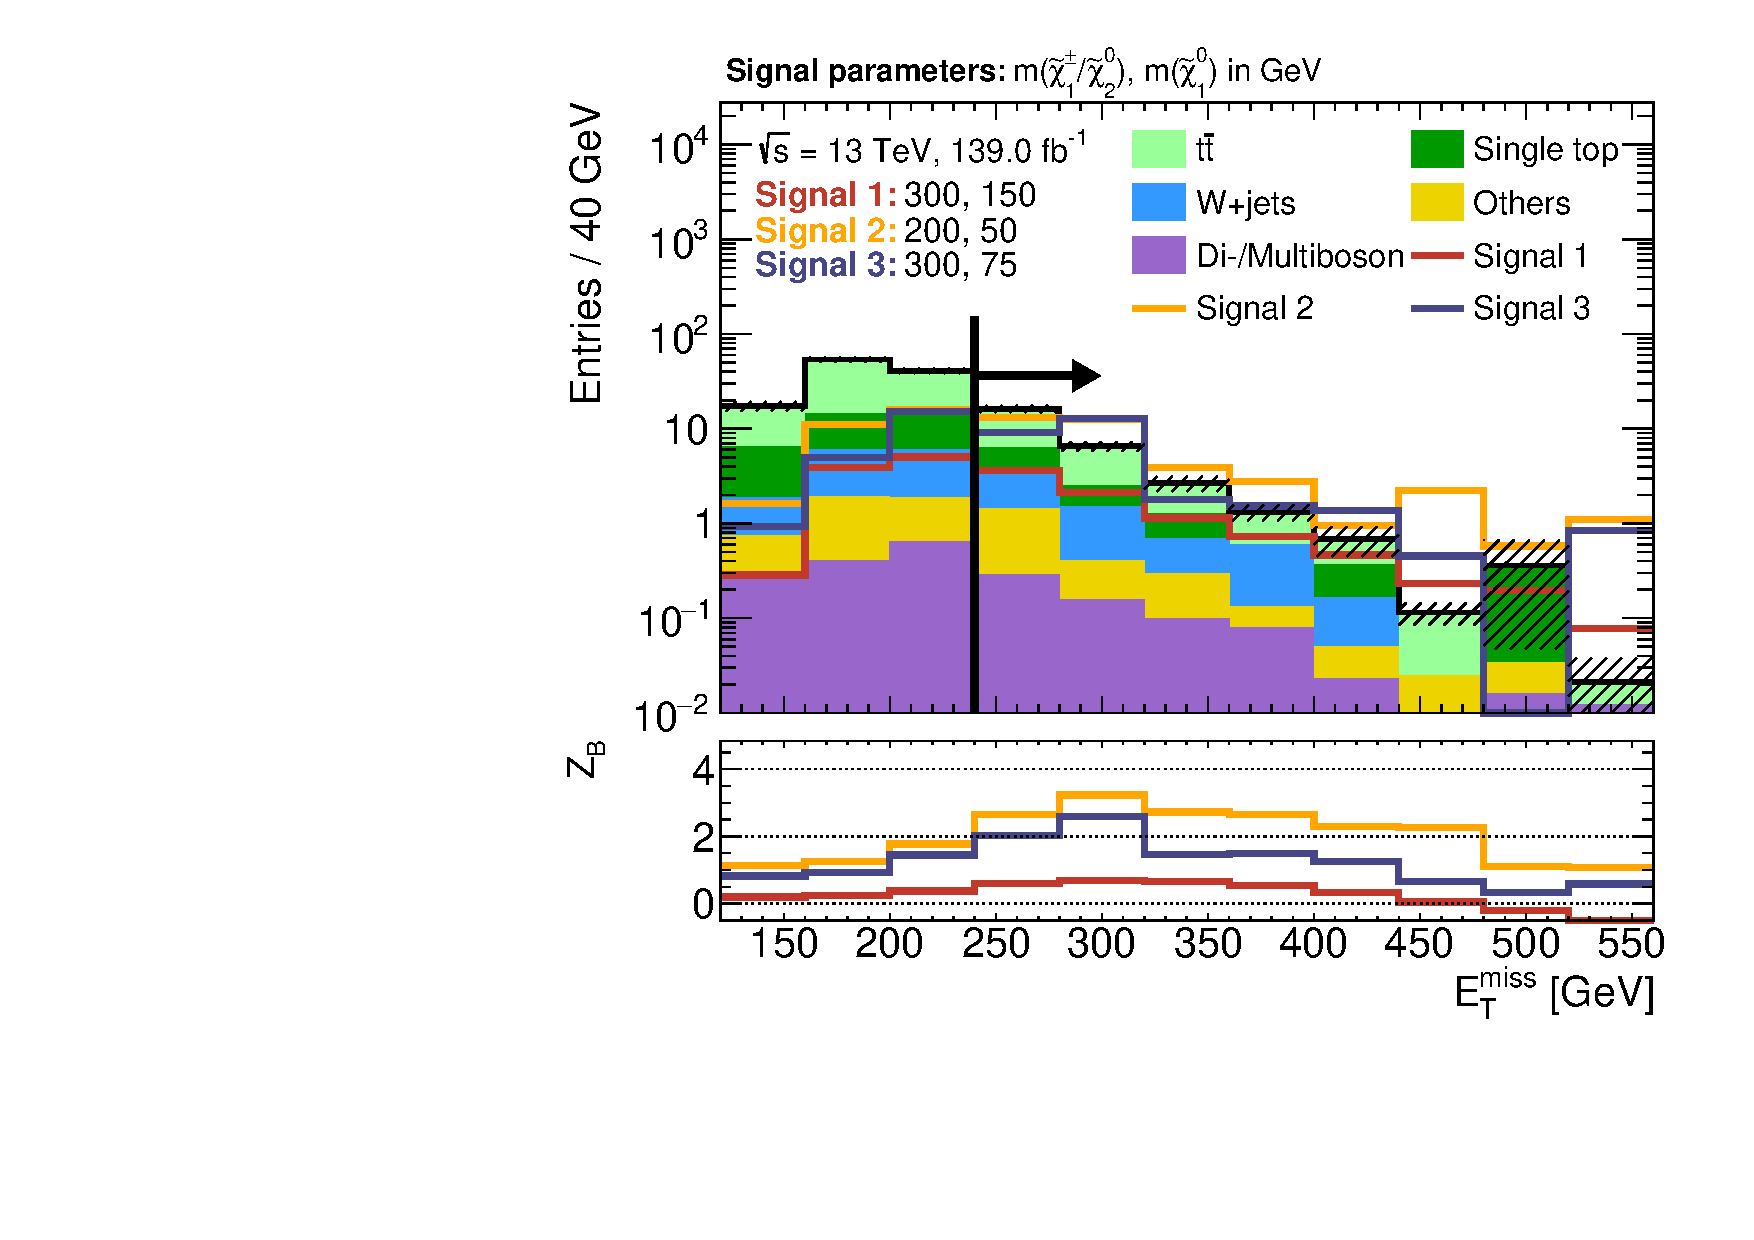
\includegraphics[width=\textwidth]{n1_SRLM_mct_bins/met.pdf}
		\caption{\label{fig:Wh_reopt_second_round_n1_srlm_met}}
	\end{subfigure}%
	\begin{subfigure}[b]{0.4\linewidth}
		\centering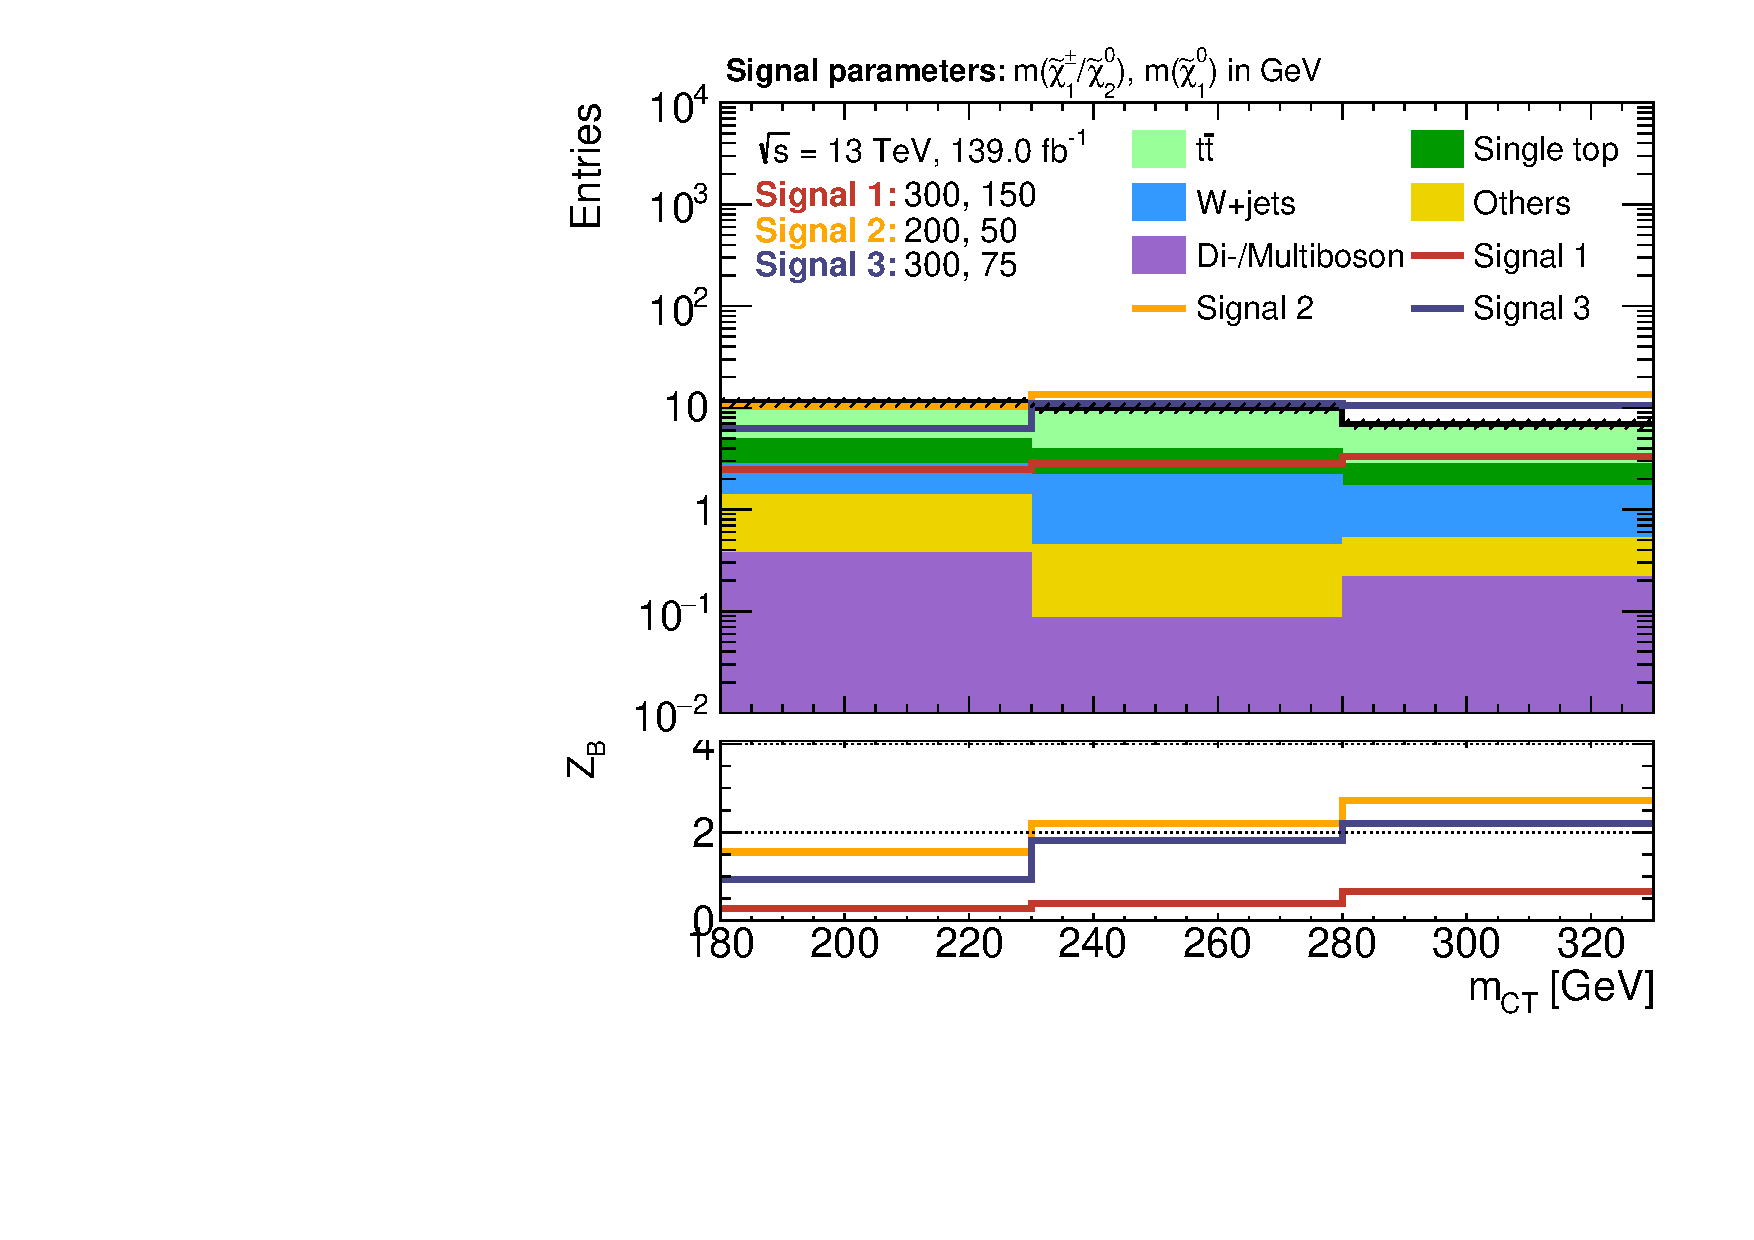
\includegraphics[width=\textwidth]{n1_SRLM_mct_bins/mct.pdf}
		\caption{\label{fig:Wh_reopt_second_round_n1_srlm_mct}}
	\end{subfigure}
	\begin{subfigure}[b]{0.4\linewidth}
		\centering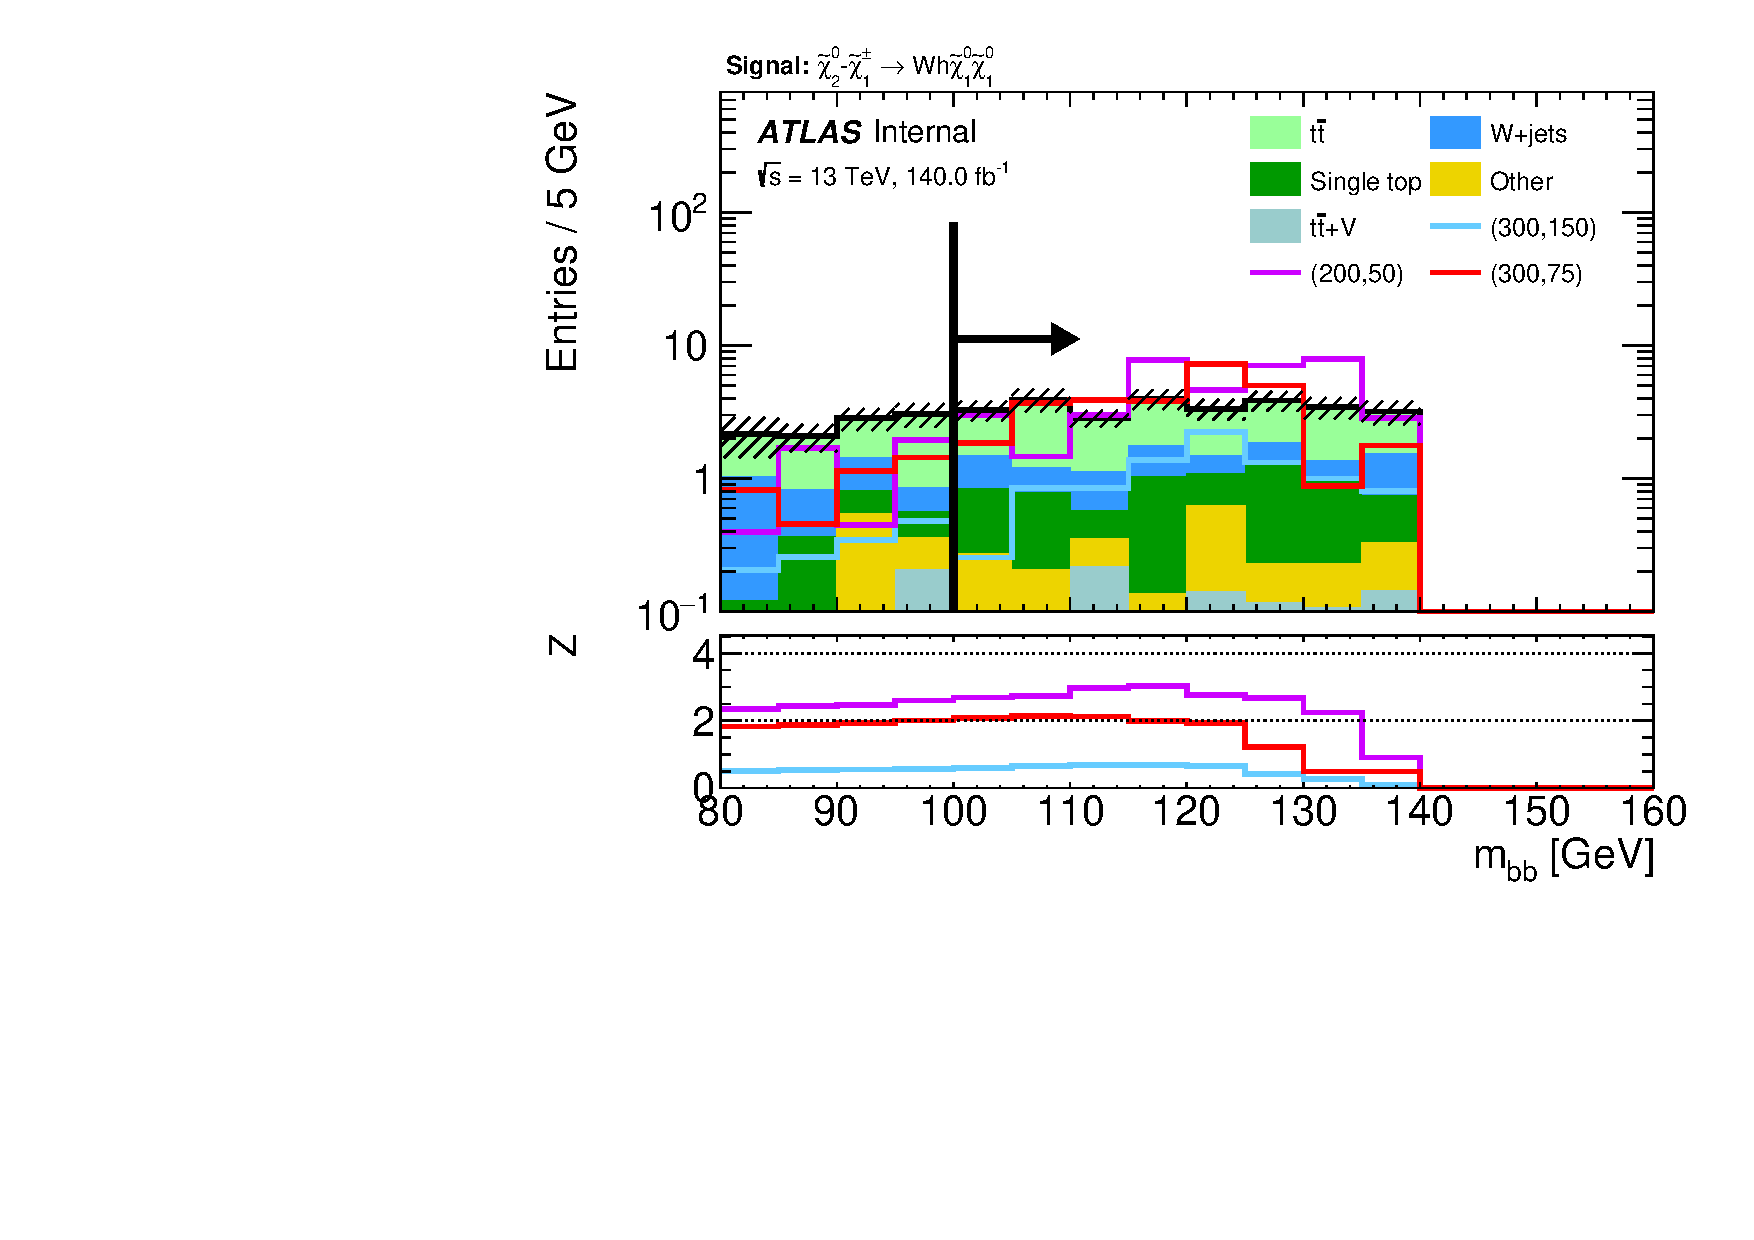
\includegraphics[width=\textwidth]{n1_SRLM_mct_bins/mbb_lower.pdf}
		\caption{\label{fig:Wh_reopt_second_round_n1_srlm_mbb_lower}}
	\end{subfigure}%
	\begin{subfigure}[b]{0.4\linewidth}
		\centering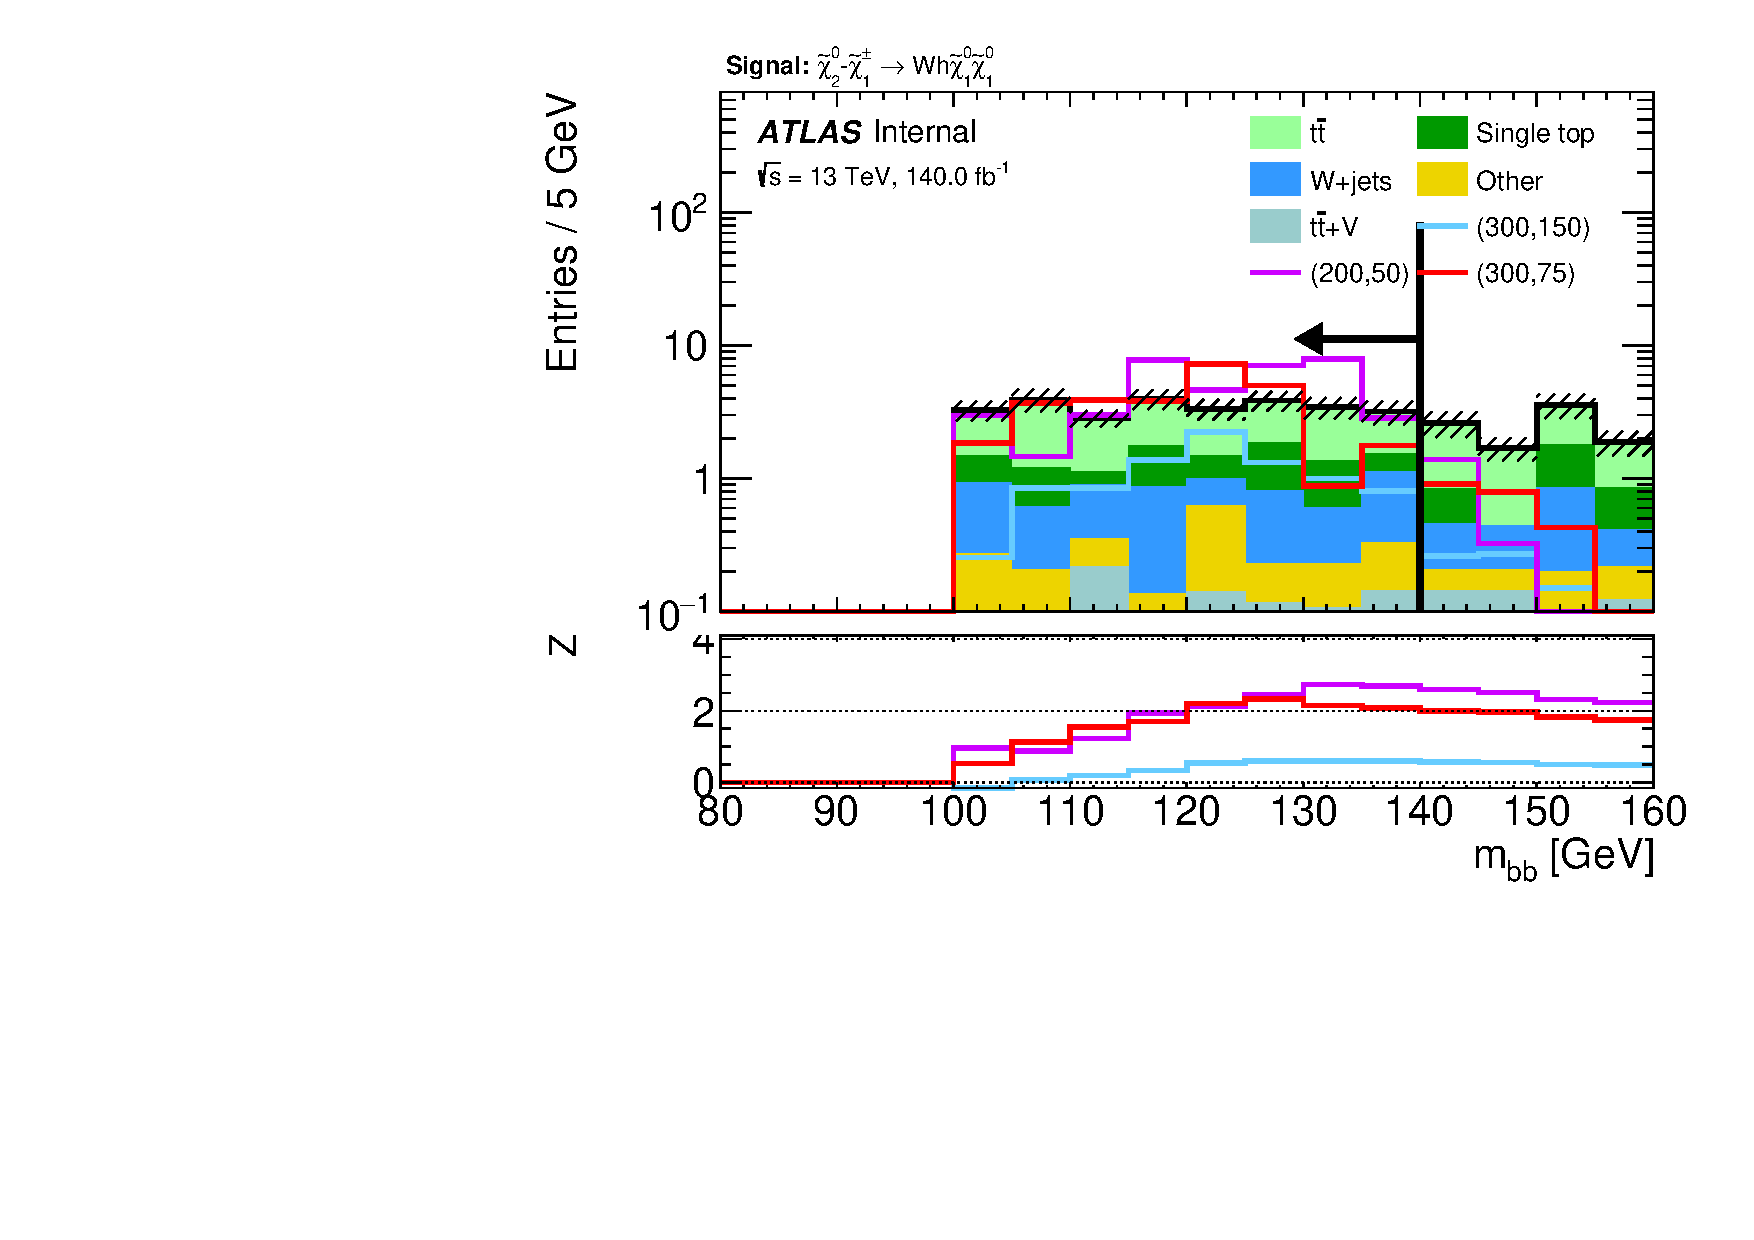
\includegraphics[width=\textwidth]{n1_SRLM_mct_bins/mbb_upper.pdf}
		\caption{\label{fig:Wh_reopt_second_round_n1_srlm_mbb_upper}}
	\end{subfigure}
	\begin{subfigure}[b]{0.4\linewidth}
		\centering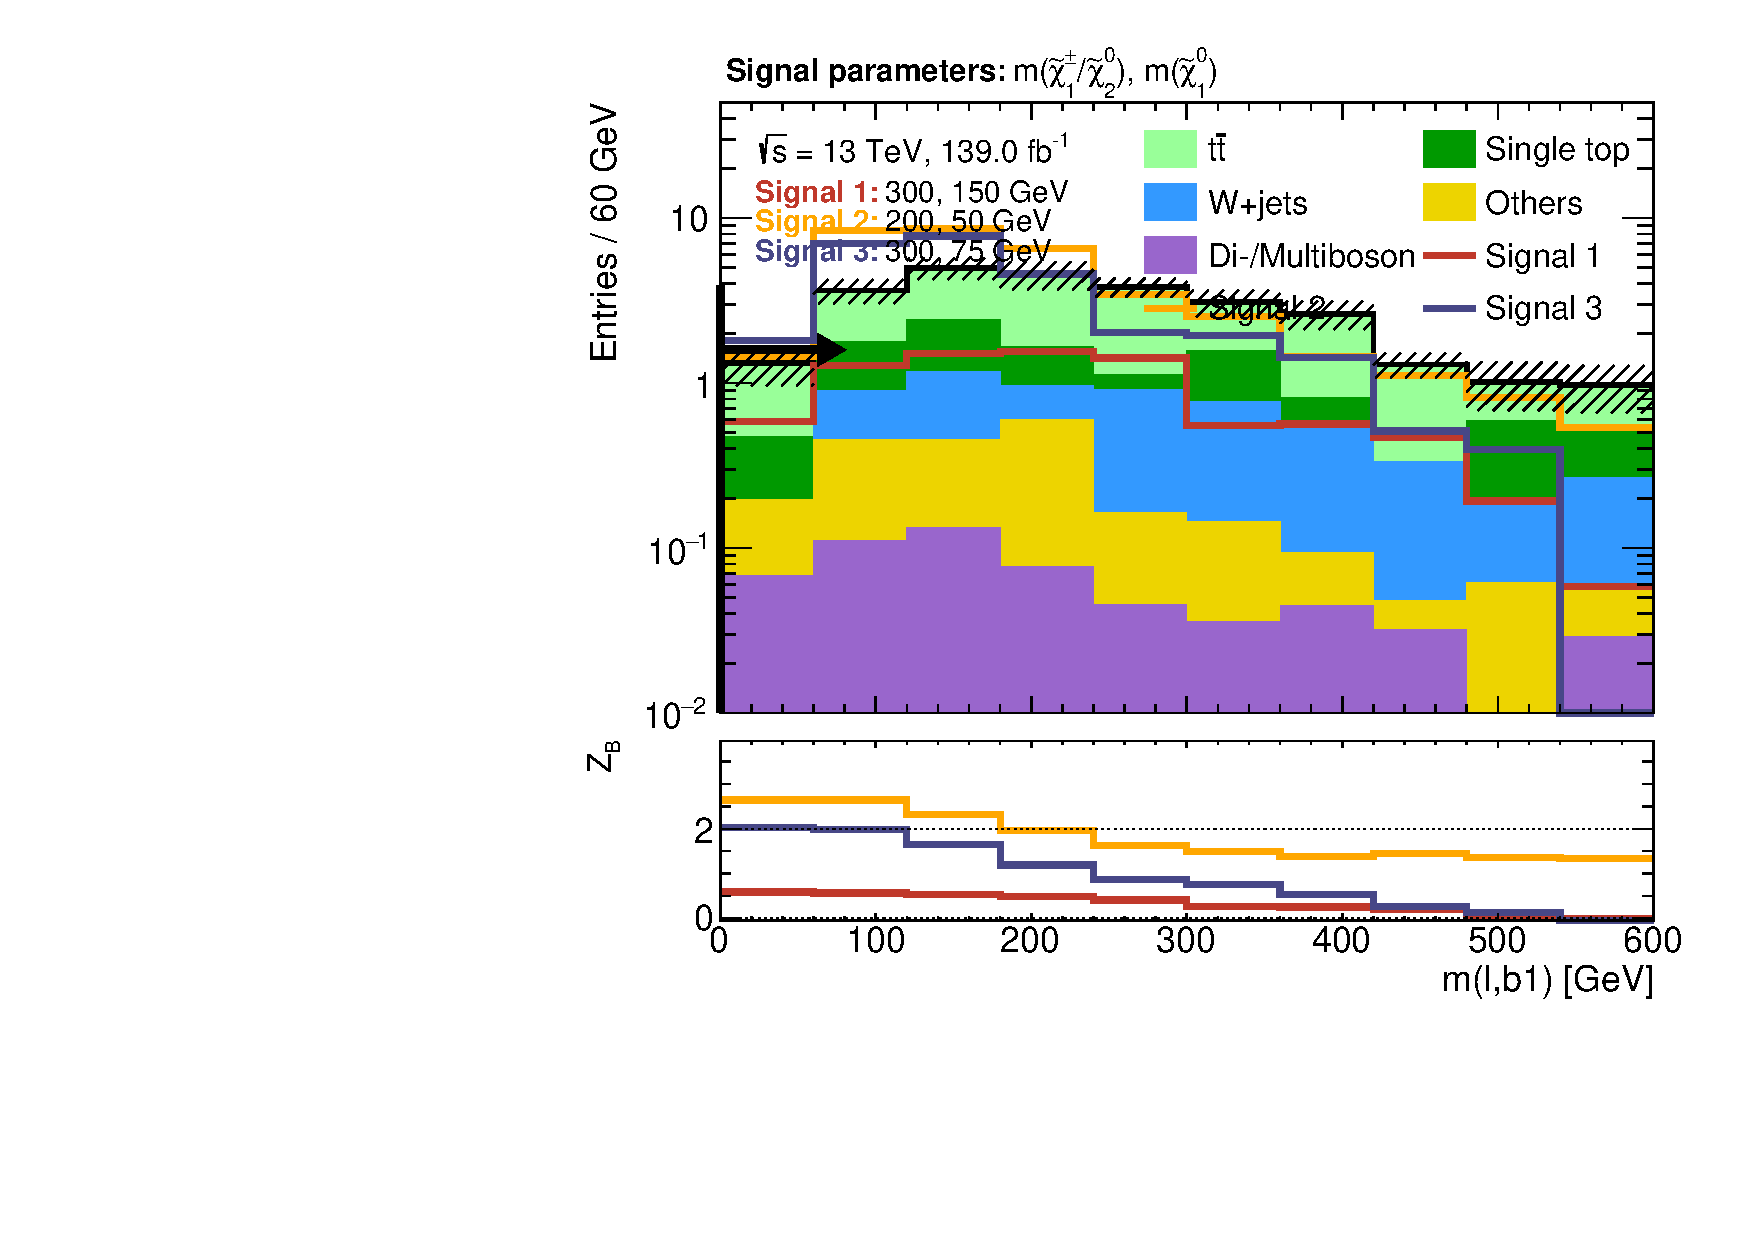
\includegraphics[width=\textwidth]{n1_SRLM_mct_bins/mlb1.pdf}
		\caption{\label{fig:Wh_reopt_second_round_n1_srlm_mlb1}}
	\end{subfigure}%
	\begin{subfigure}[b]{0.4\linewidth}
		\centering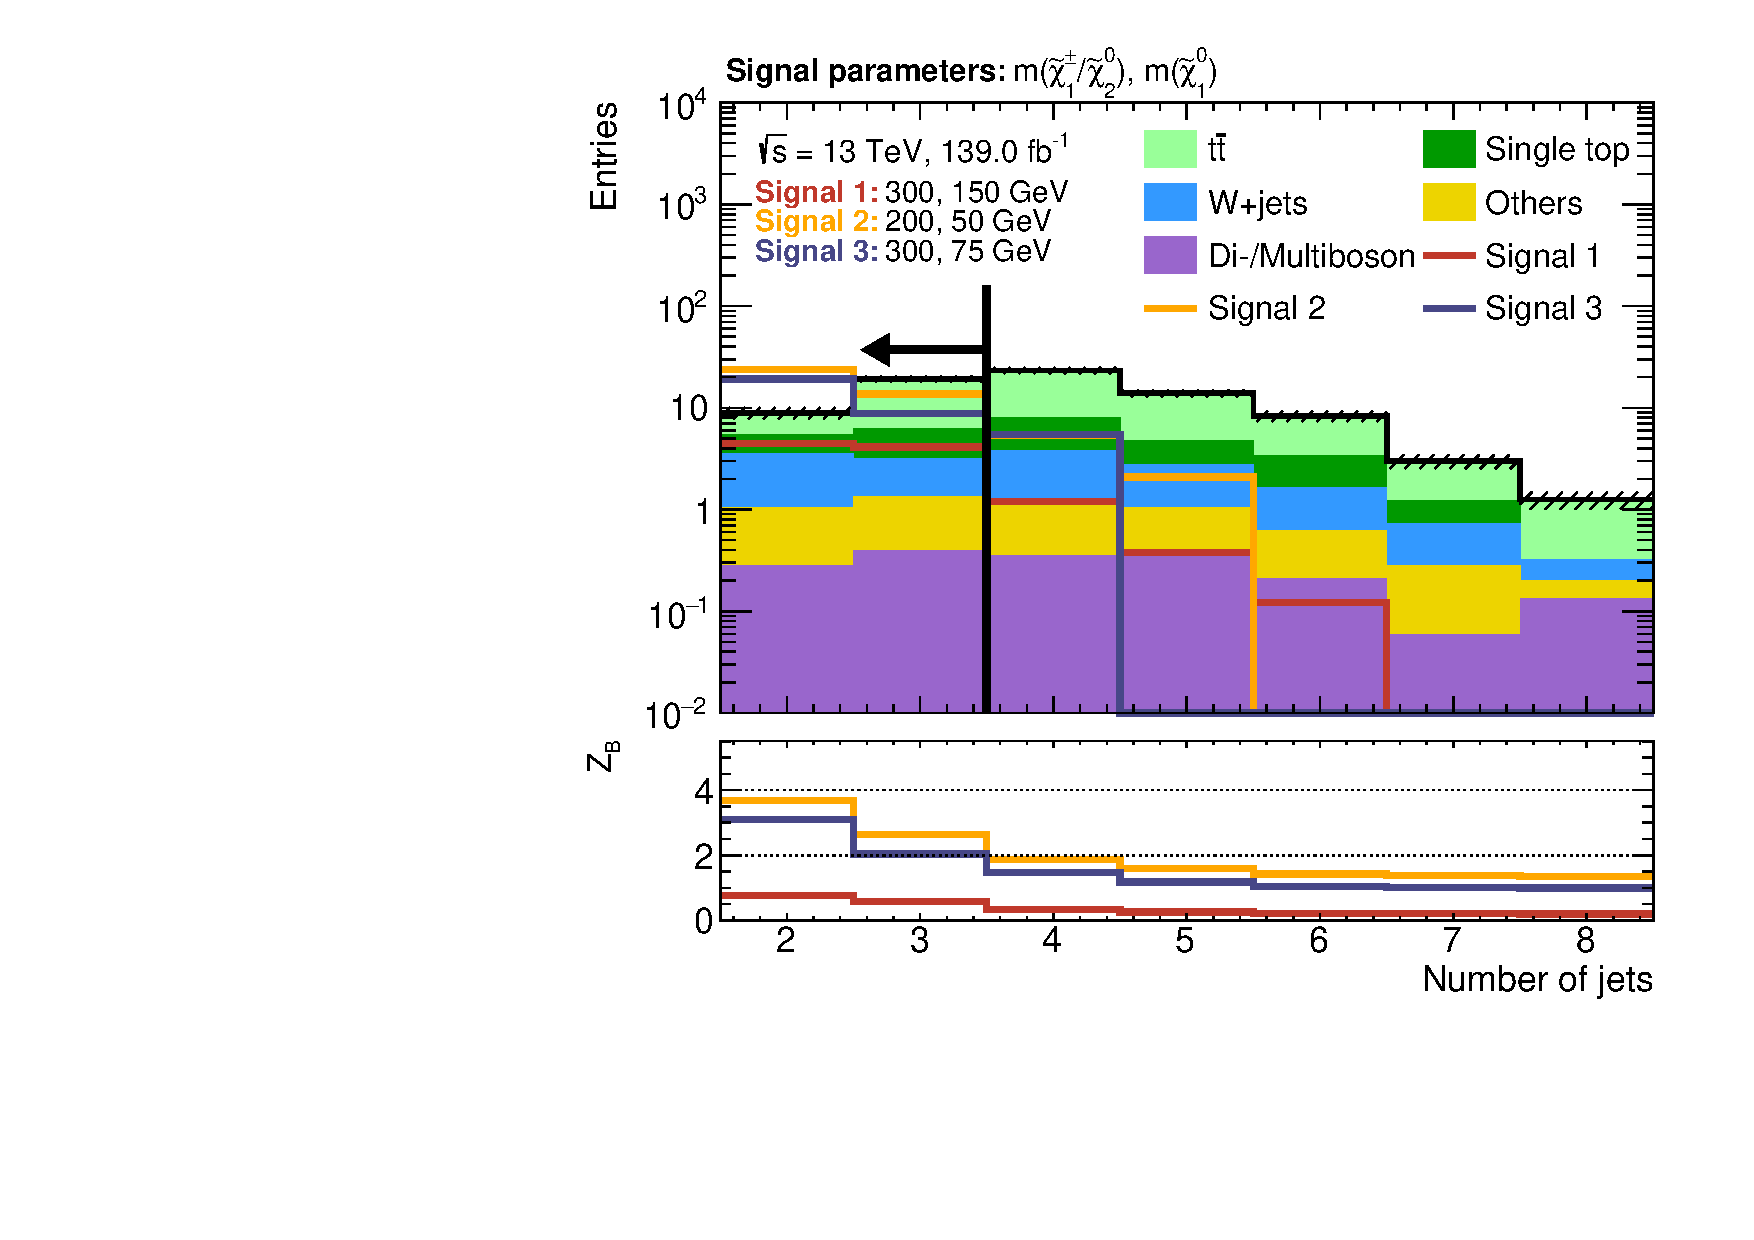
\includegraphics[width=\textwidth]{n1_SRLM_mct_bins/nJet30.pdf}
		\caption{\label{fig:Wh_reopt_second_round_n1_srlm_njet}}
	\end{subfigure}
	\caption{N-1 plots for the SR LM, with exemplary signal points and all $\mct$ bins included. In all figures except \figname~\subref{fig:Wh_reopt_second_round_n1_srlm_mct}, the significance in the lower pad is obtained by summing up all the events in the direction of the cut arrow and includes 30\% uncertainty as well as MC statistical uncertainty. In \figname~\subref{fig:Wh_reopt_second_round_n1_srlm_mct} the significance is only computed on a bin-by-bin basis, \ie not summing up all events in the direction of the cut arrow.}
	\label{fig:Wh_reopt_second_round_n1_srlm}
\end{figure}

\begin{figure}
	\centering
	\begin{subfigure}[b]{0.4\linewidth}
		\centering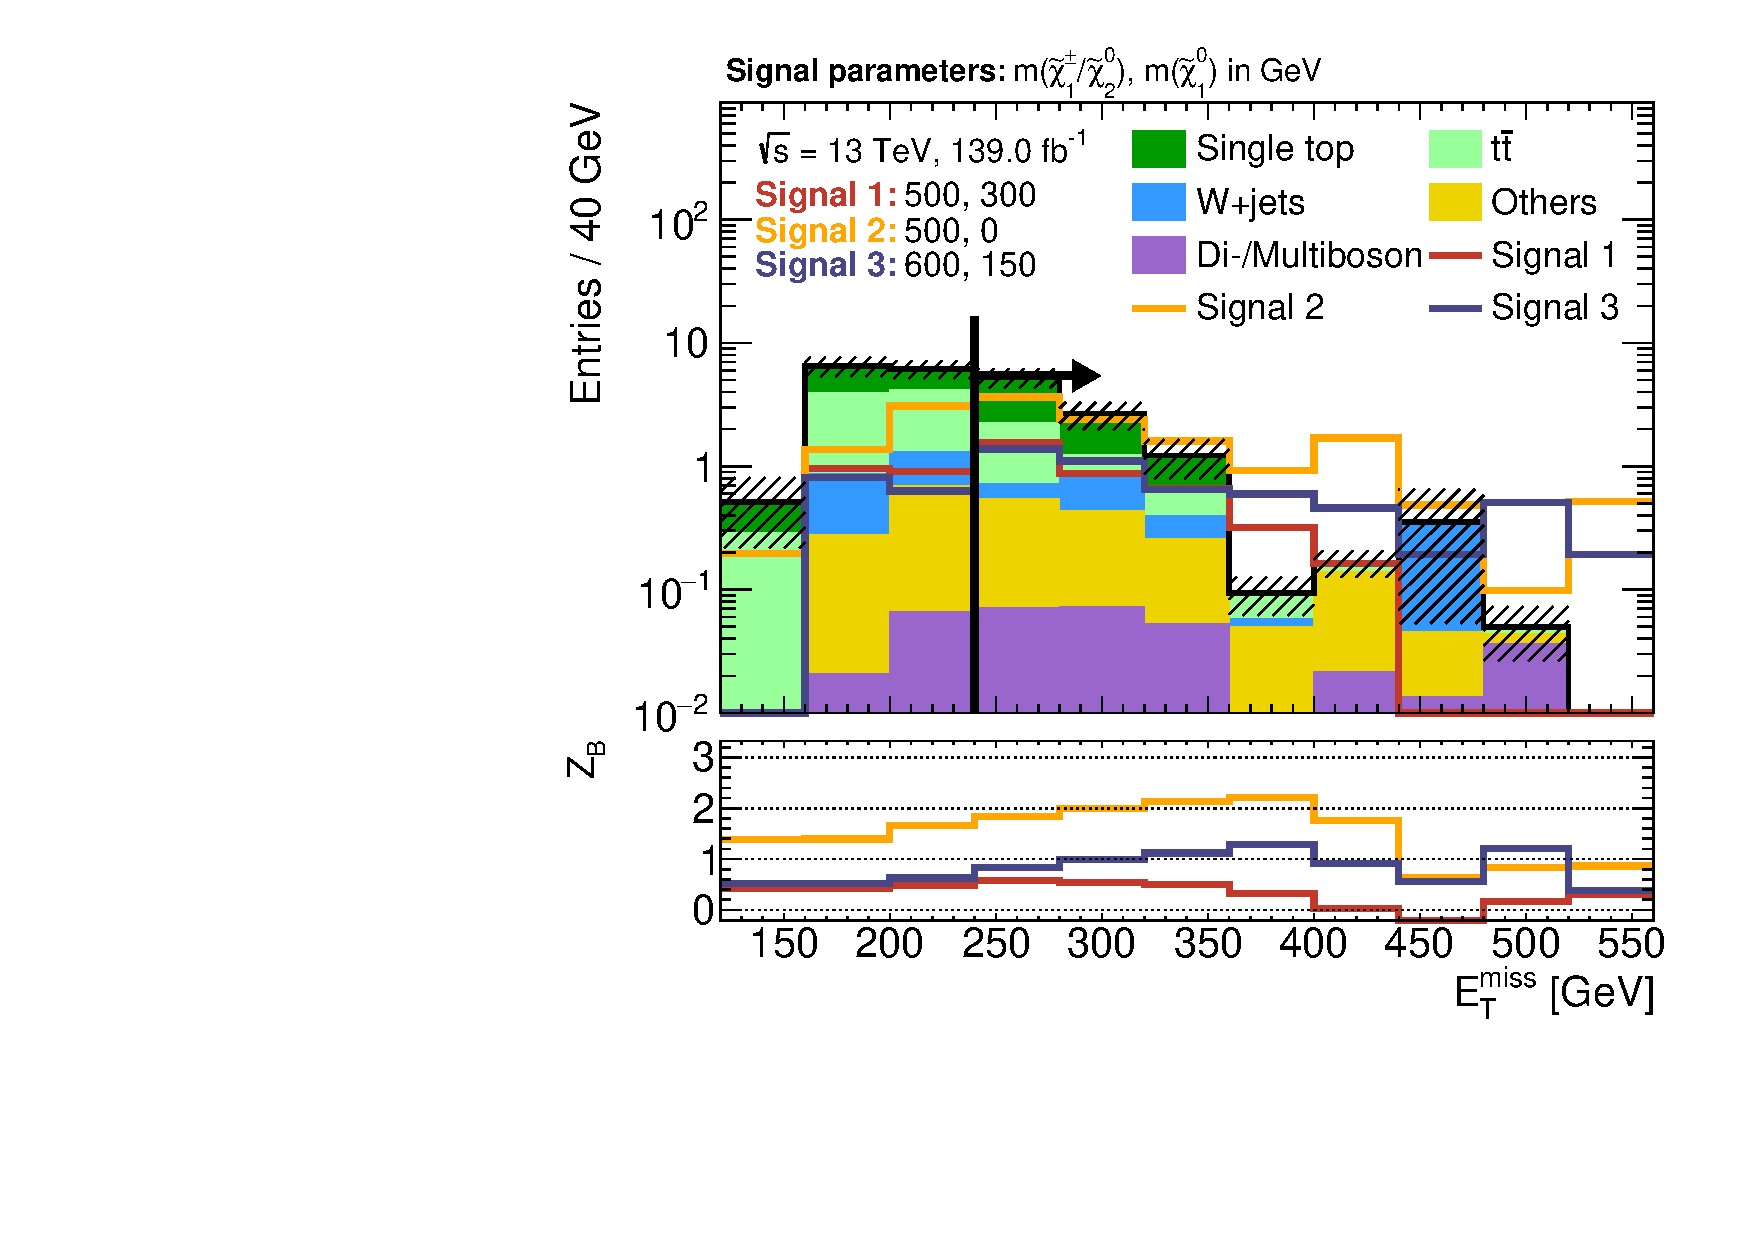
\includegraphics[width=\textwidth]{n1_SRMM_mct_bins/met.pdf}
		\caption{\label{fig:Wh_reopt_second_round_n1_srmm_met}}
	\end{subfigure}%
	\begin{subfigure}[b]{0.4\linewidth}
		\centering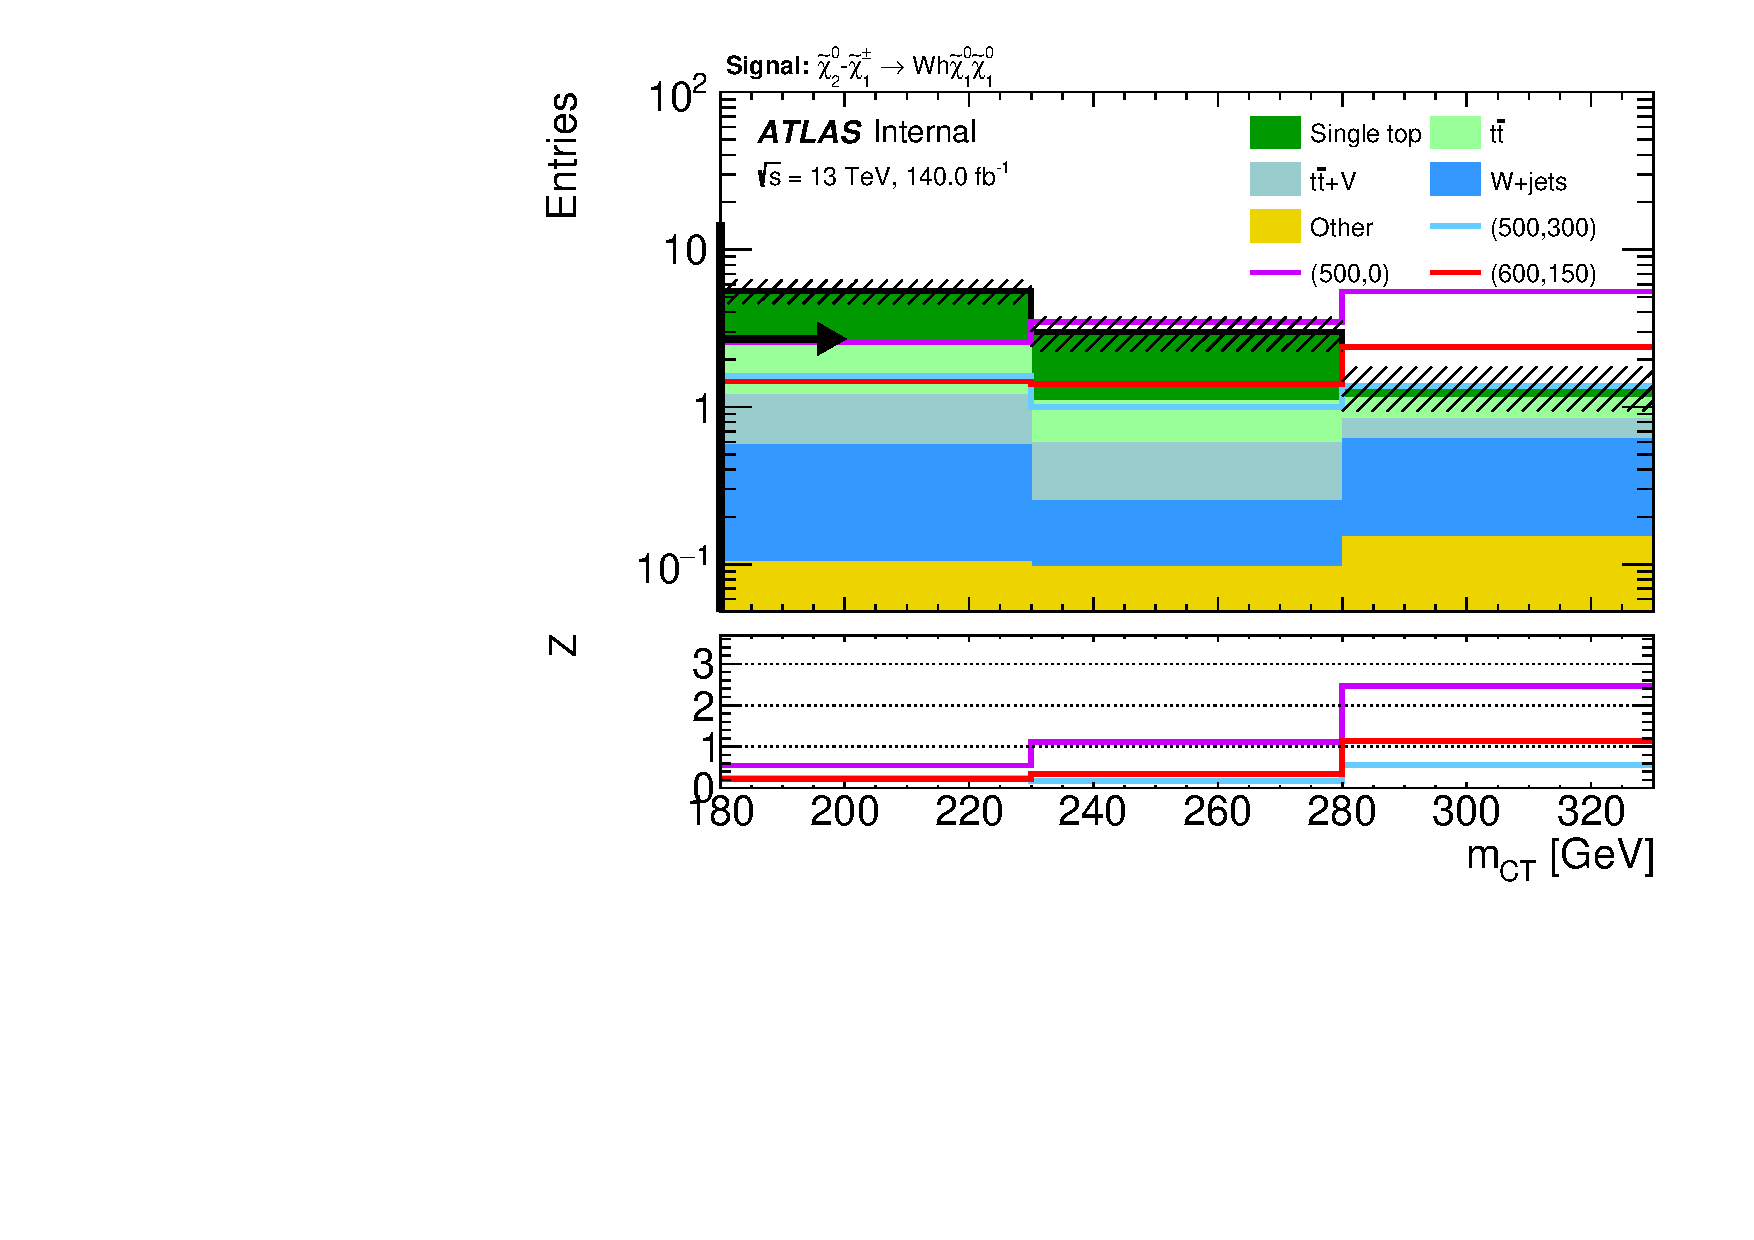
\includegraphics[width=\textwidth]{n1_SRMM_mct_bins/mct.pdf}
		\caption{\label{fig:Wh_reopt_second_round_n1_srmm_mct}}
	\end{subfigure}
	\begin{subfigure}[b]{0.4\linewidth}
		\centering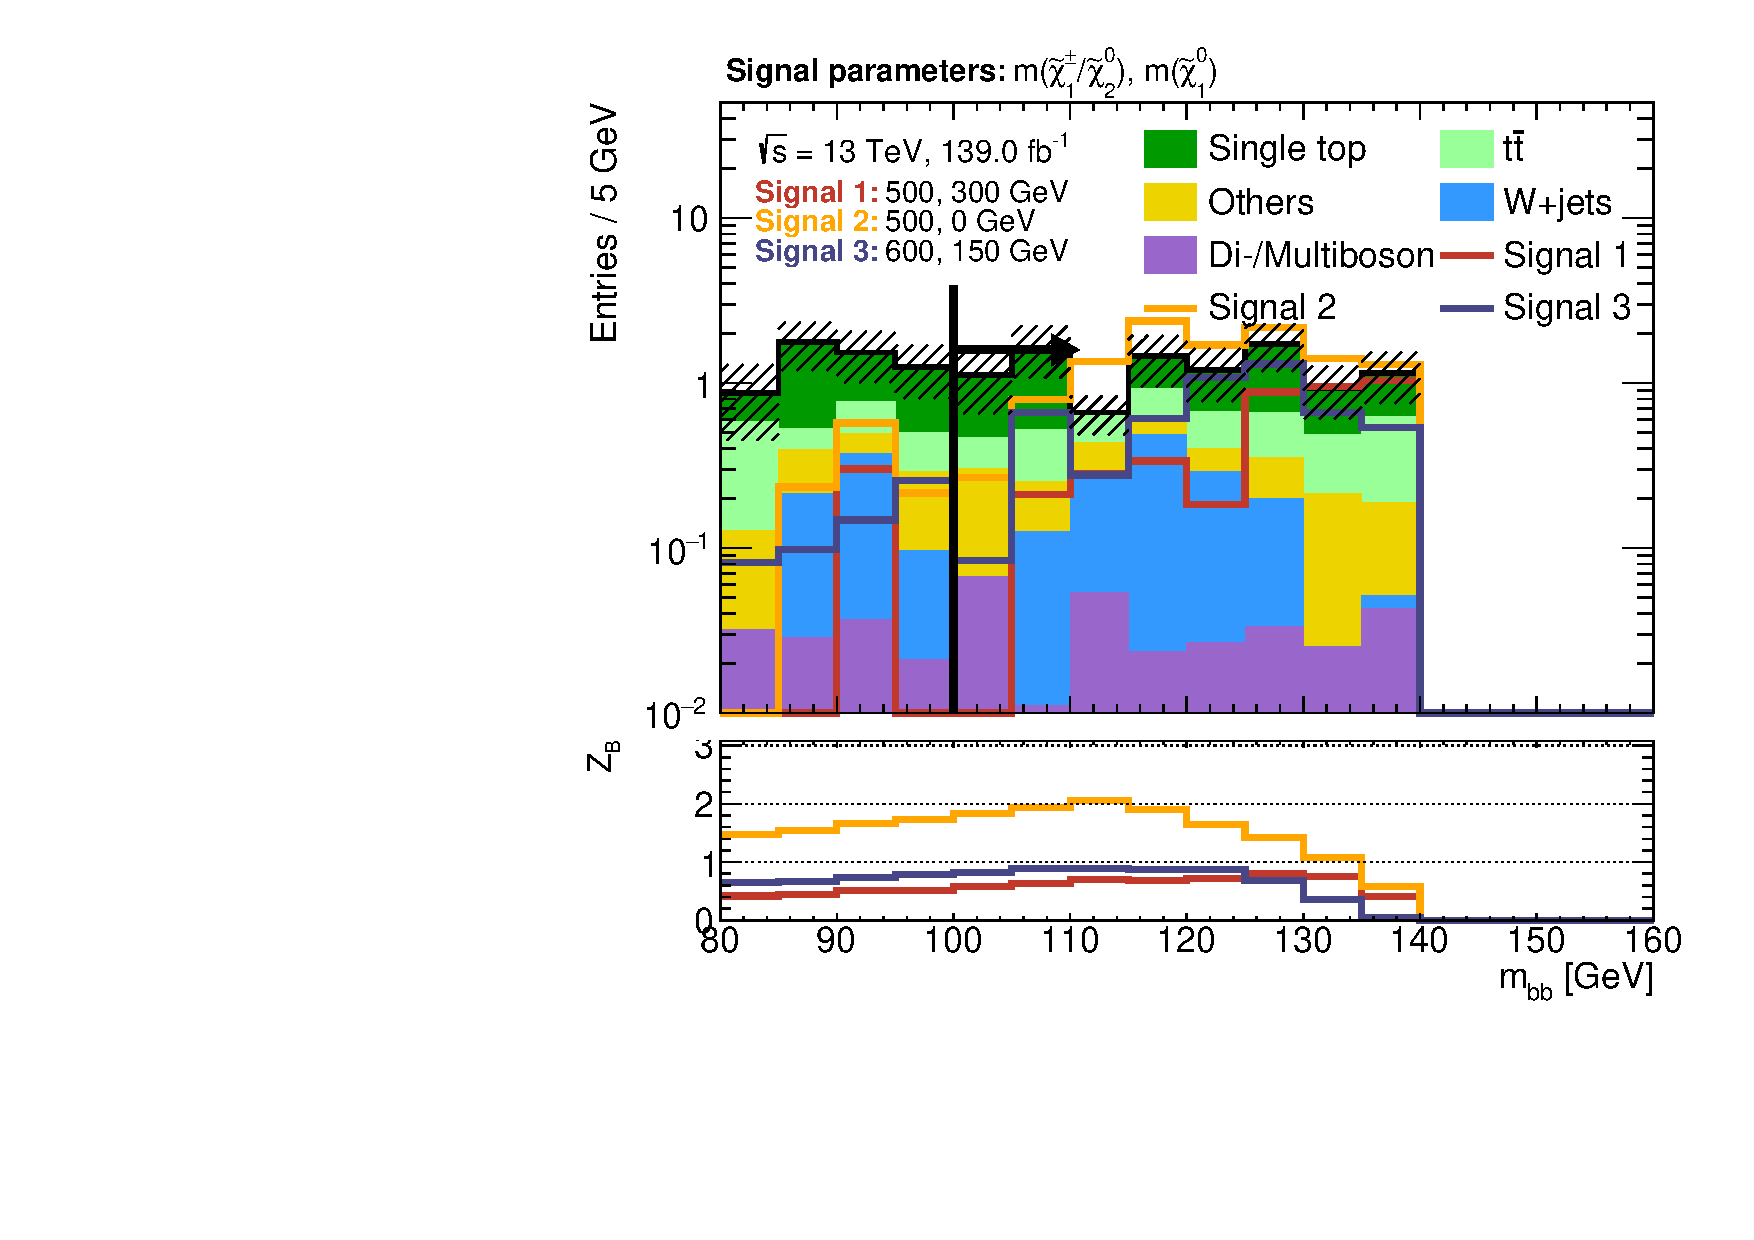
\includegraphics[width=\textwidth]{n1_SRMM_mct_bins/mbb_lower.pdf}
		\caption{\label{fig:Wh_reopt_second_round_n1_srmm_mbb_lower}}
	\end{subfigure}%
	\begin{subfigure}[b]{0.4\linewidth}
		\centering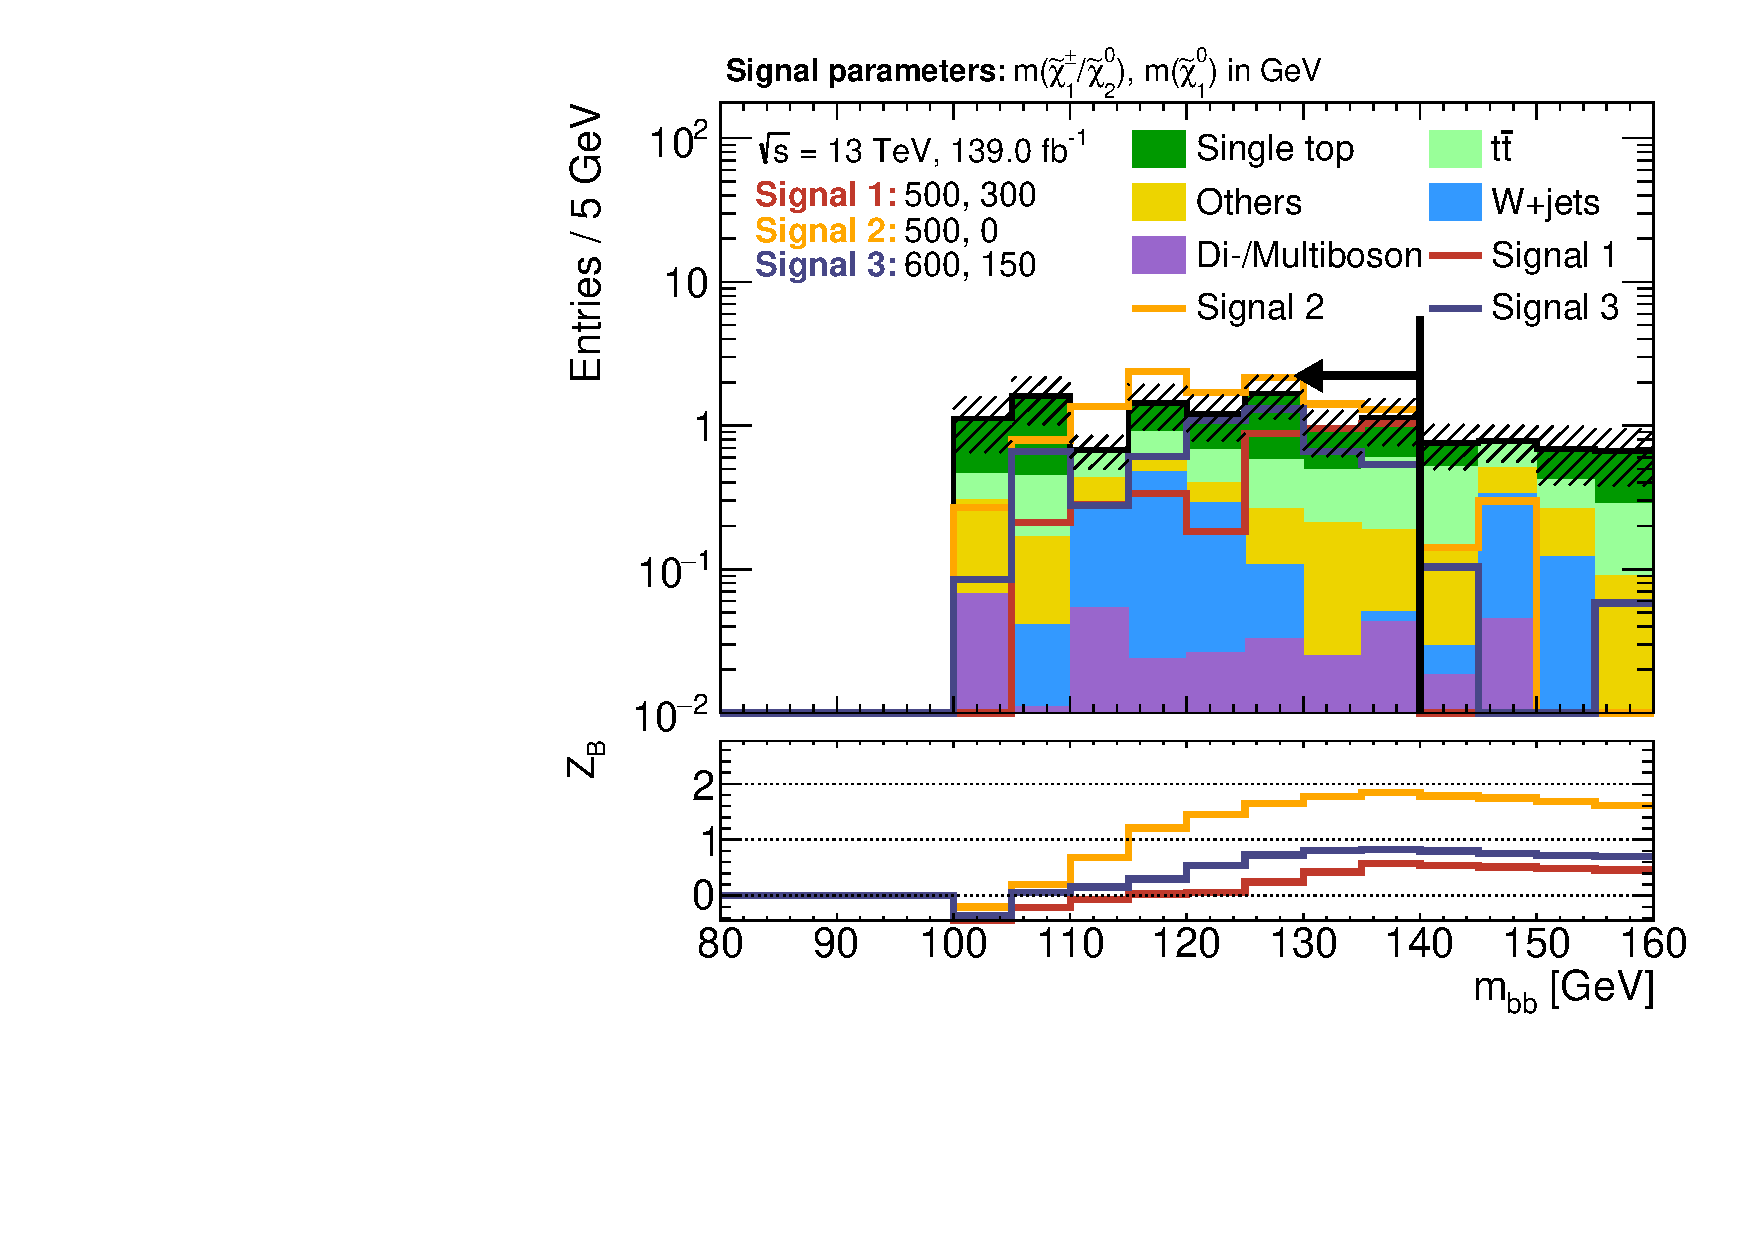
\includegraphics[width=\textwidth]{n1_SRMM_mct_bins/mbb_upper.pdf}
		\caption{\label{fig:Wh_reopt_second_round_n1_srmm_mbb_upper}}
	\end{subfigure}
	\begin{subfigure}[b]{0.4\linewidth}
		\centering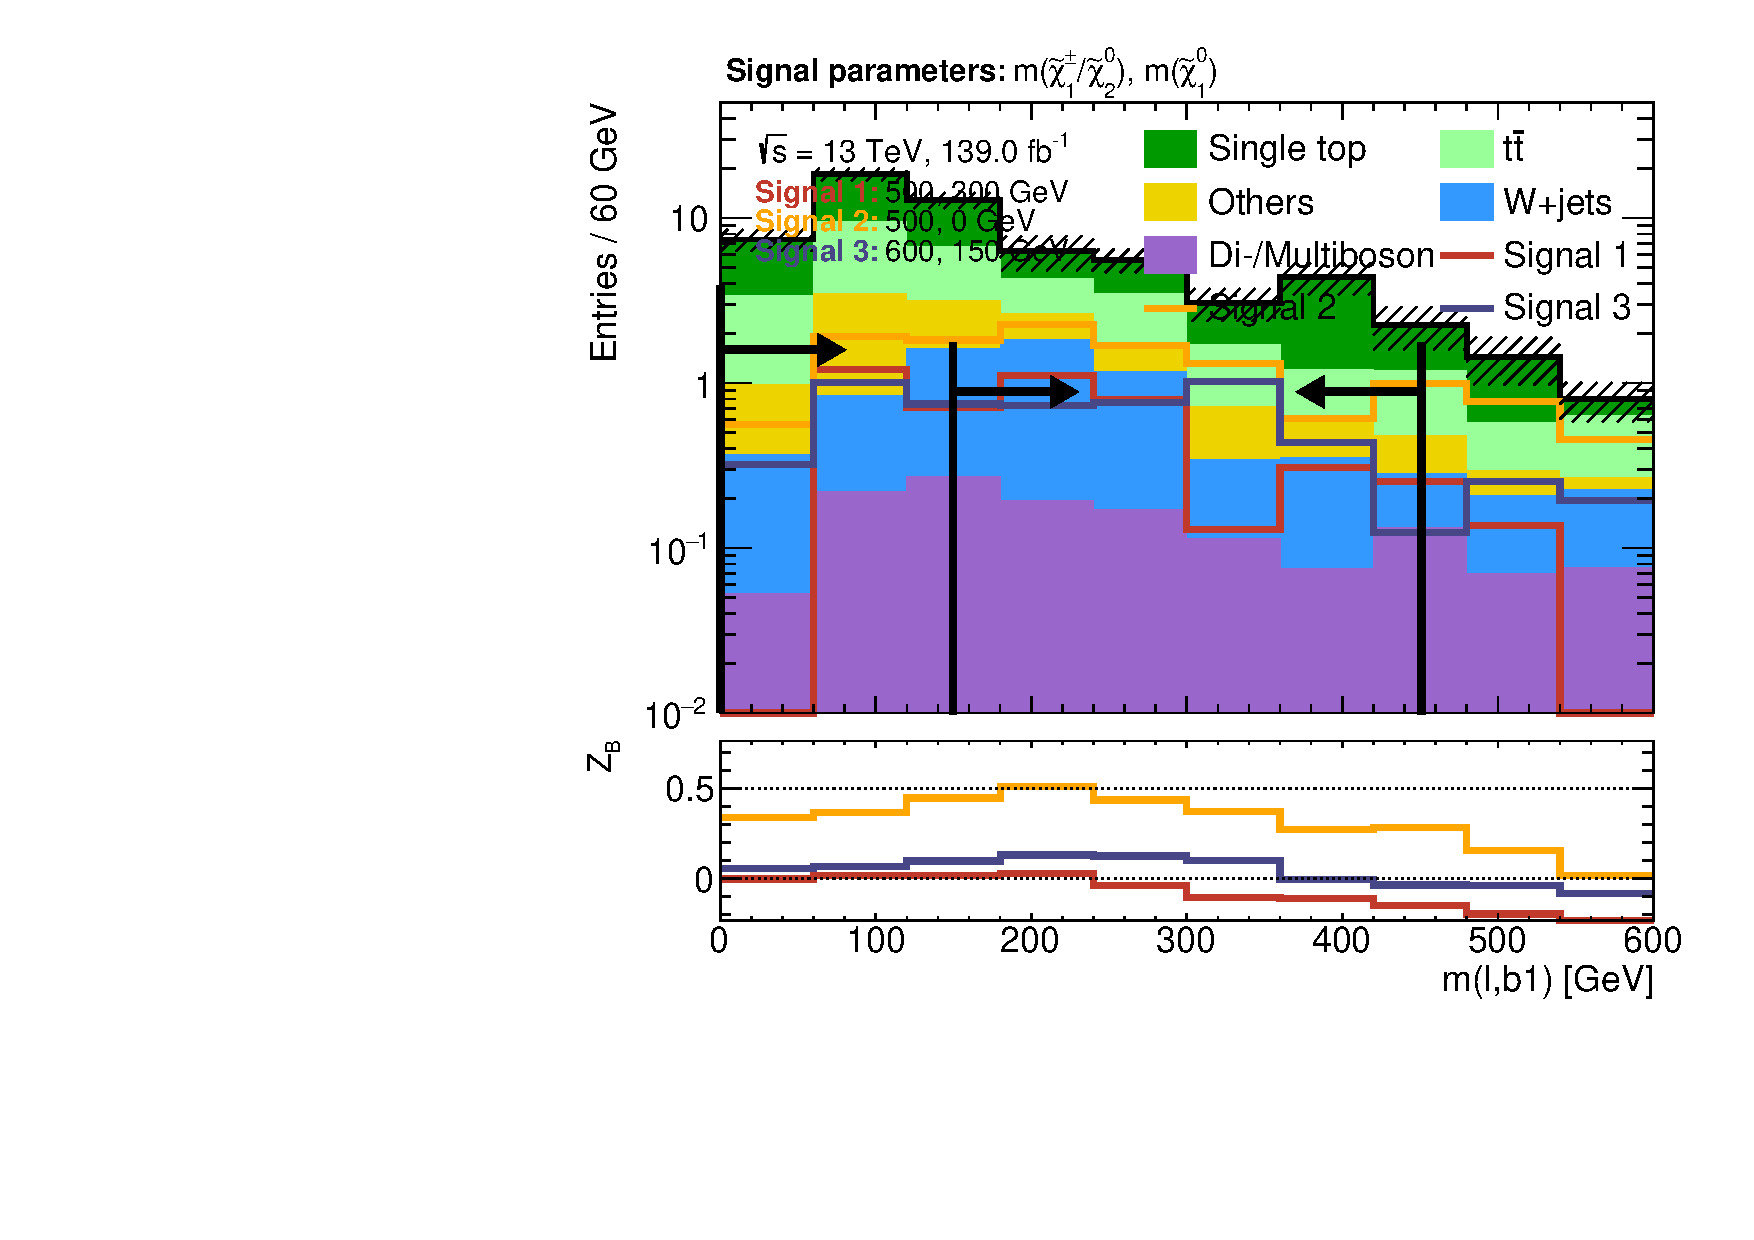
\includegraphics[width=\textwidth]{n1_SRMM_mct_bins/mlb1.pdf}
		\caption{\label{fig:Wh_reopt_second_round_n1_srmm_mlb1}}
	\end{subfigure}%
	\begin{subfigure}[b]{0.4\linewidth}
		\centering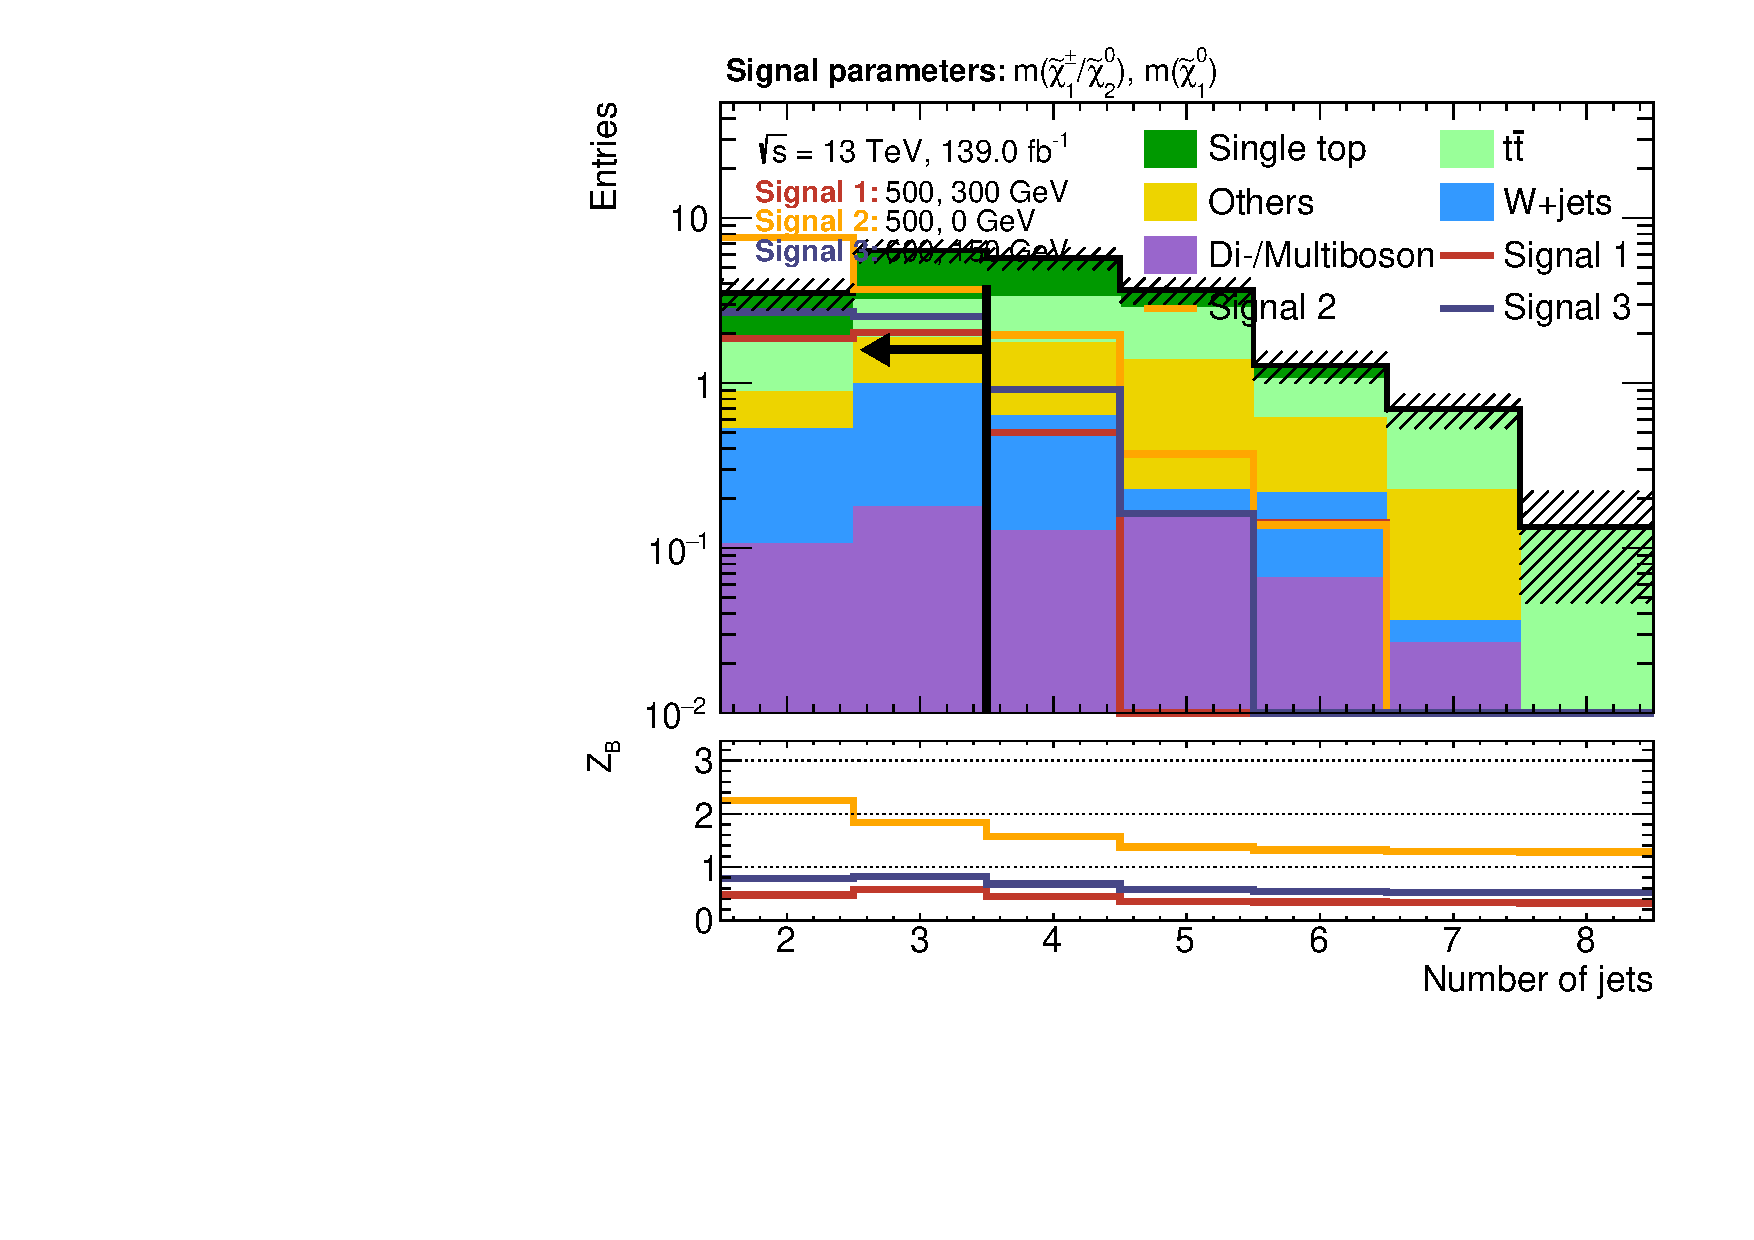
\includegraphics[width=\textwidth]{n1_SRMM_mct_bins/nJet30.pdf}
		\caption{\label{fig:Wh_reopt_second_round_n1_srmm_njet}}
	\end{subfigure}
	\caption{N-1 plots for the SR MM, with exemplary signal points and all $\mct$ bins included. In all figures except \figname~\subref{fig:Wh_reopt_second_round_n1_srmm_mct}, the significance in the lower pad is obtained by summing up all the events in the direction of the cut arrow and includes 30\% uncertainty as well as MC statistical uncertainty. In \figname~\subref{fig:Wh_reopt_second_round_n1_srmm_mct} the significance is only computed on a bin-by-bin basis, \ie not summing up all events in the direction of the cut arrow.}
	\label{fig:Wh_reopt_second_round_n1_srmm}
\end{figure}

\begin{figure}
	\centering
	\begin{subfigure}[b]{0.4\linewidth}
		\centering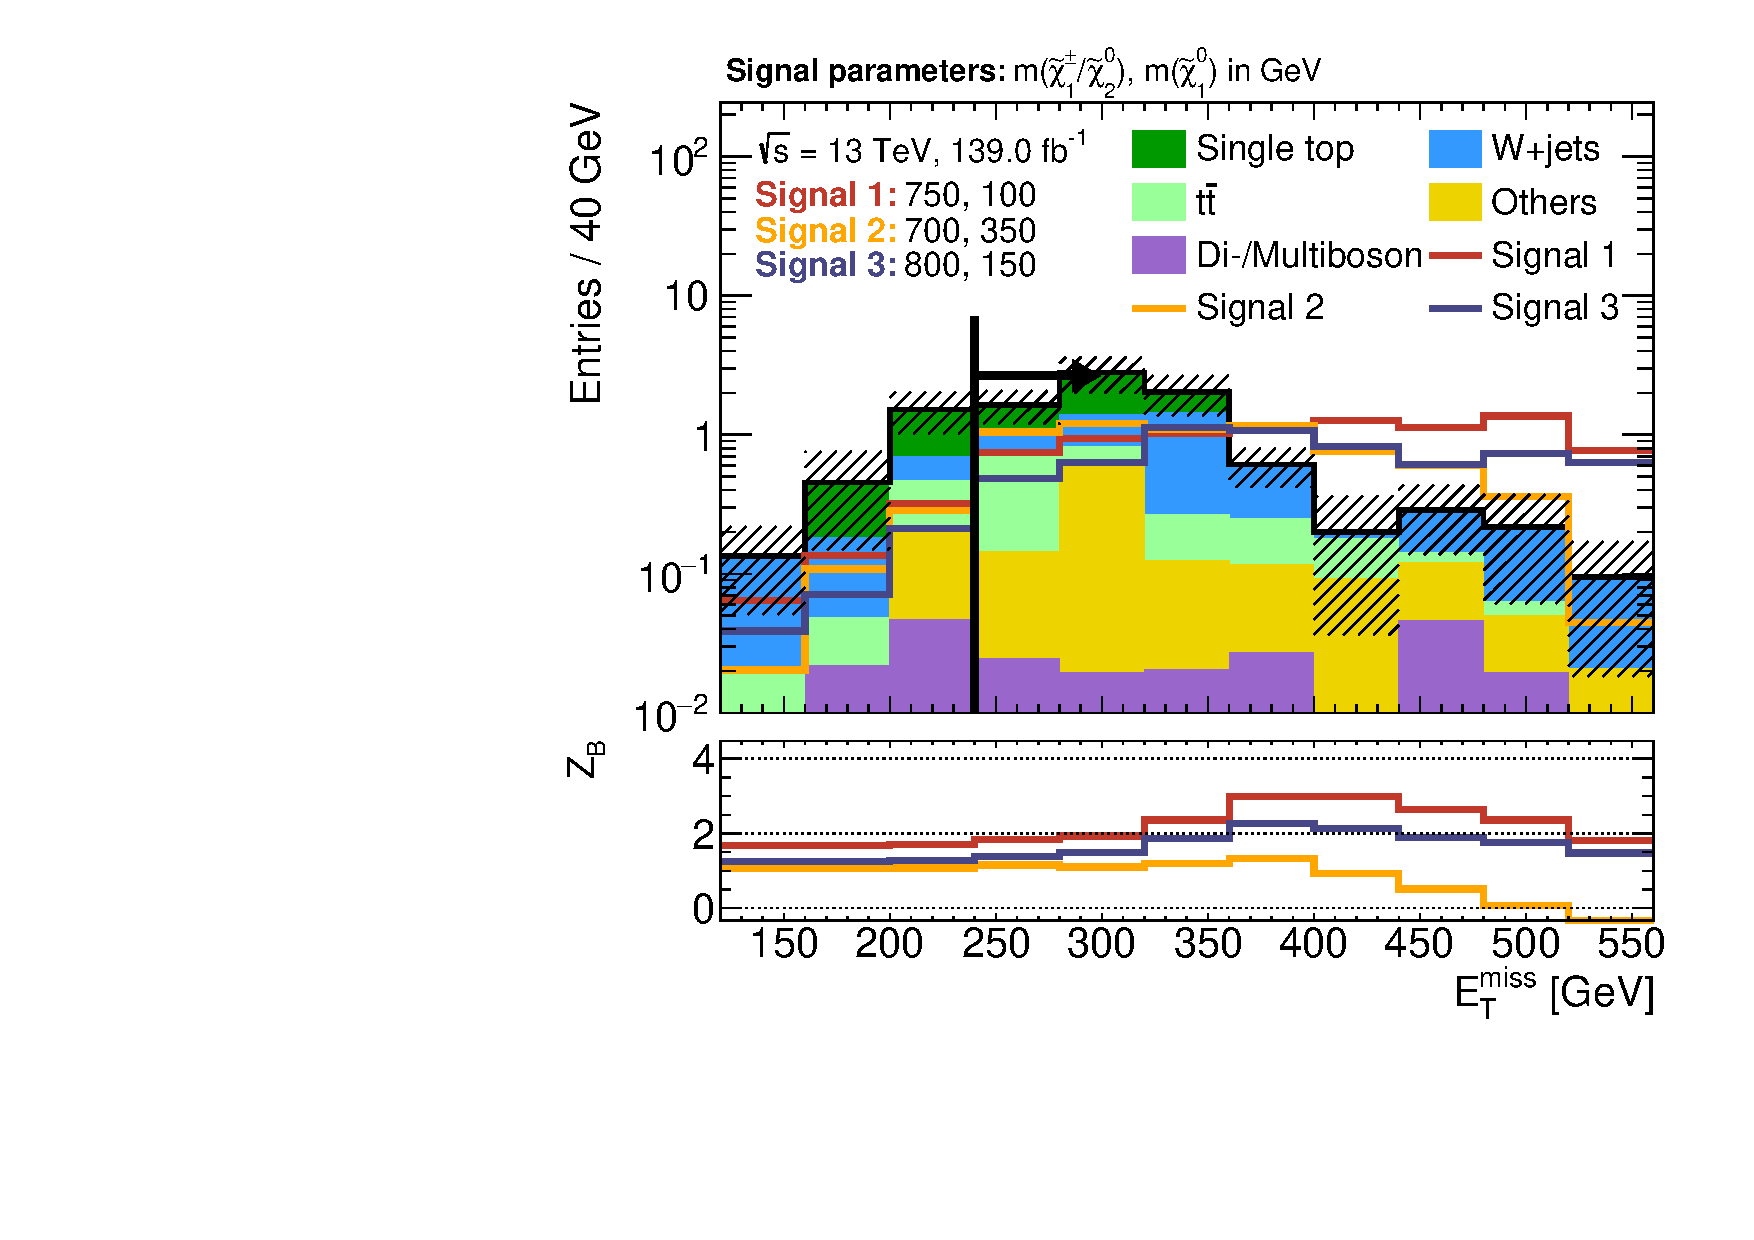
\includegraphics[width=\textwidth]{n1_SRHM_mct_bins/met.pdf}
		\caption{\label{fig:Wh_reopt_second_round_n1_srhm_met}}
	\end{subfigure}%
	\begin{subfigure}[b]{0.4\linewidth}
		\centering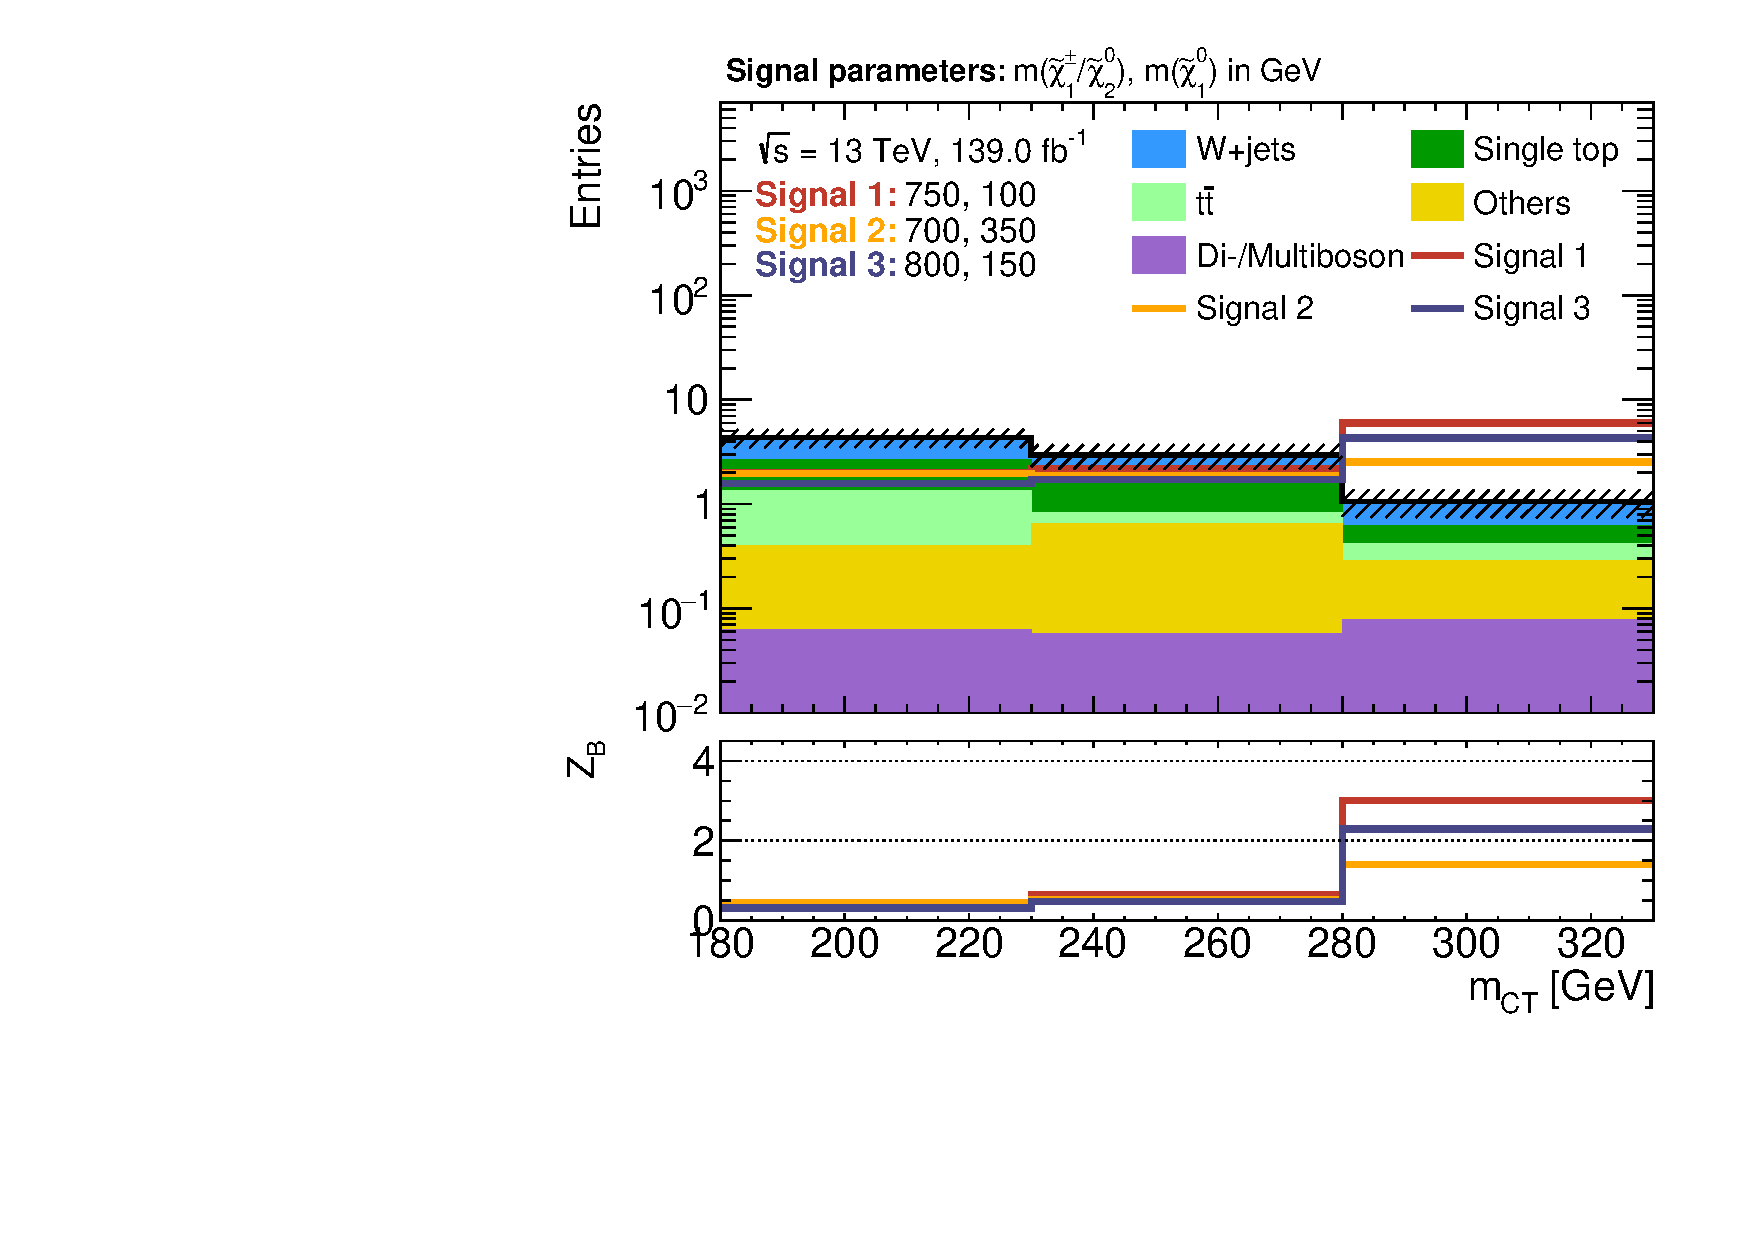
\includegraphics[width=\textwidth]{n1_SRHM_mct_bins/mct.pdf}
		\caption{\label{fig:Wh_reopt_second_round_n1_srhm_mct}}
	\end{subfigure}
	\begin{subfigure}[b]{0.4\linewidth}
		\centering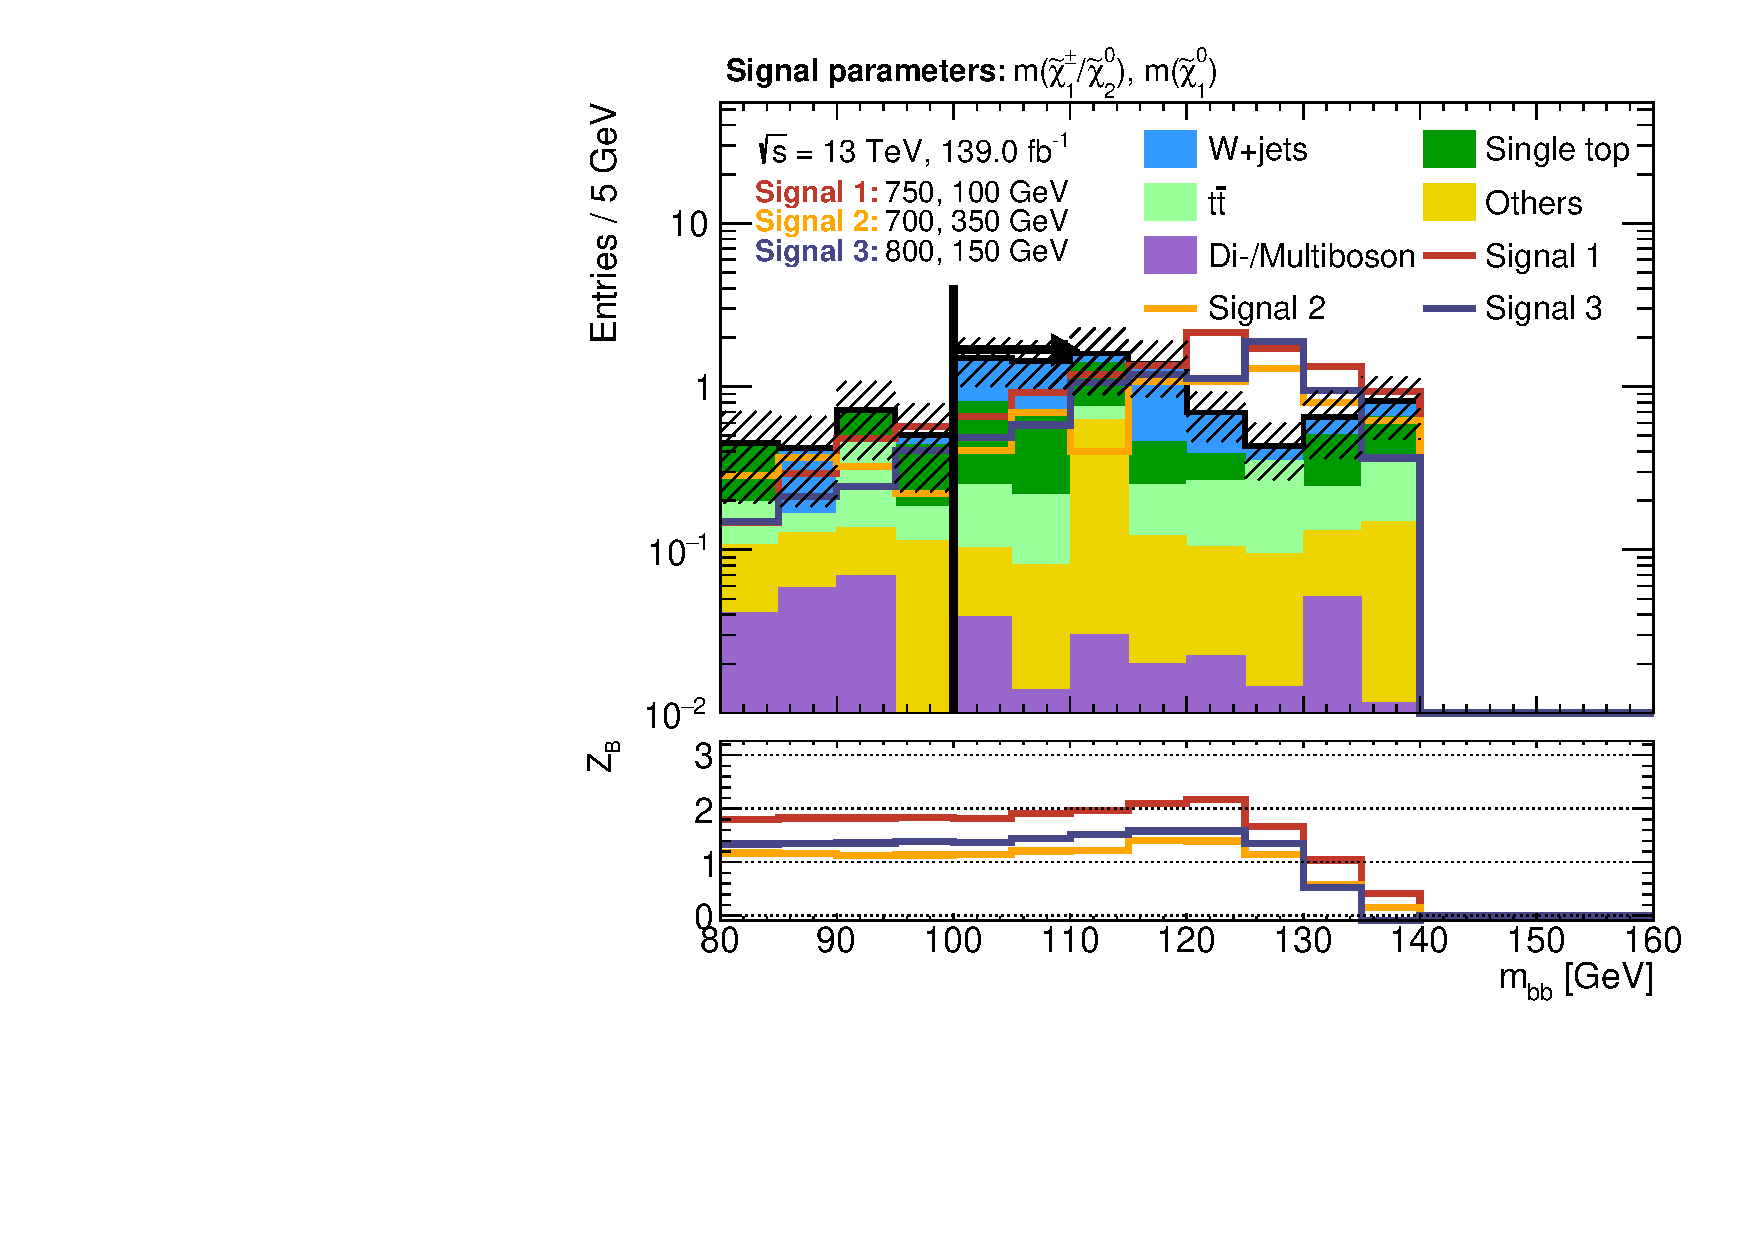
\includegraphics[width=\textwidth]{n1_SRHM_mct_bins/mbb_lower.pdf}
		\caption{\label{fig:Wh_reopt_second_round_n1_srhm_mbb_lower}}
	\end{subfigure}%
	\begin{subfigure}[b]{0.4\linewidth}
		\centering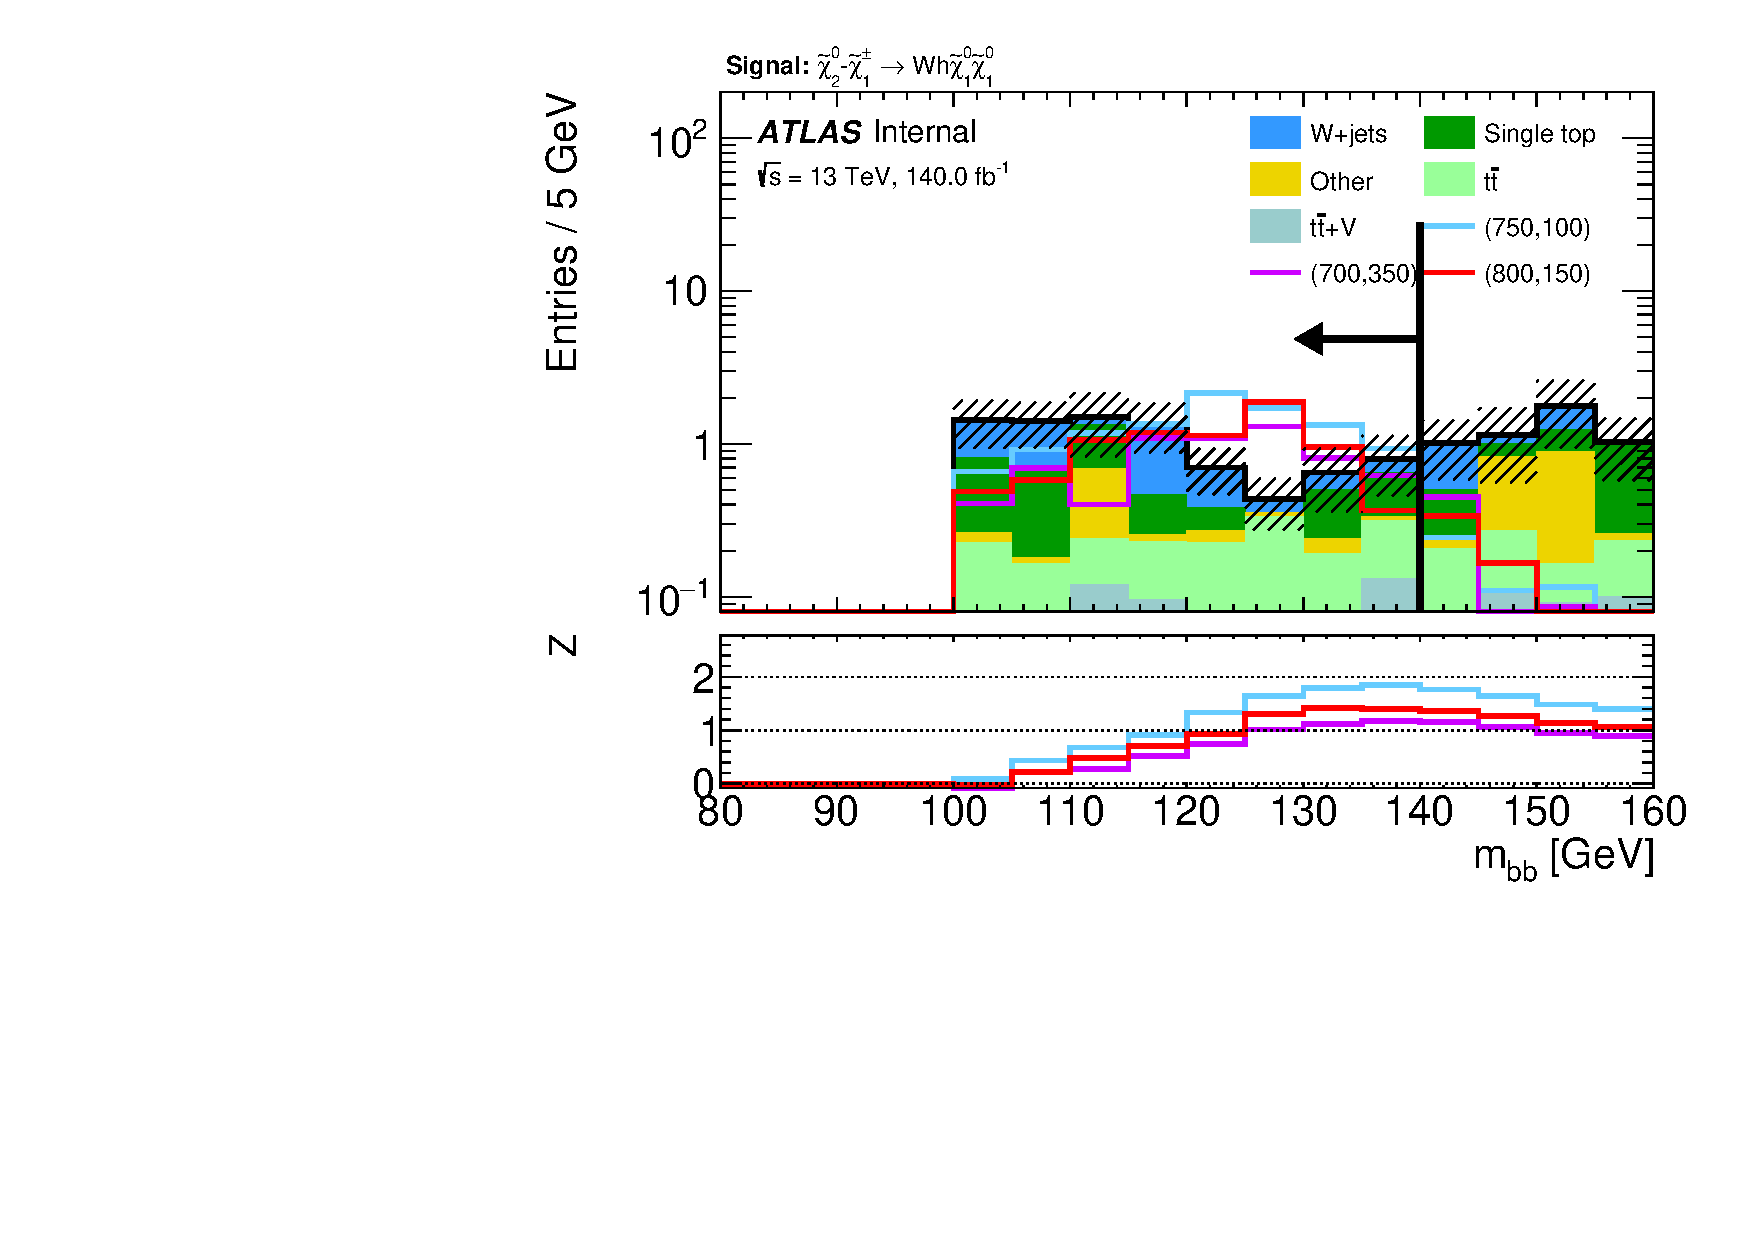
\includegraphics[width=\textwidth]{n1_SRHM_mct_bins/mbb_upper.pdf}
		\caption{\label{fig:Wh_reopt_second_round_n1_srhm_mbb_upper}}
	\end{subfigure}
	\begin{subfigure}[b]{0.4\linewidth}
		\centering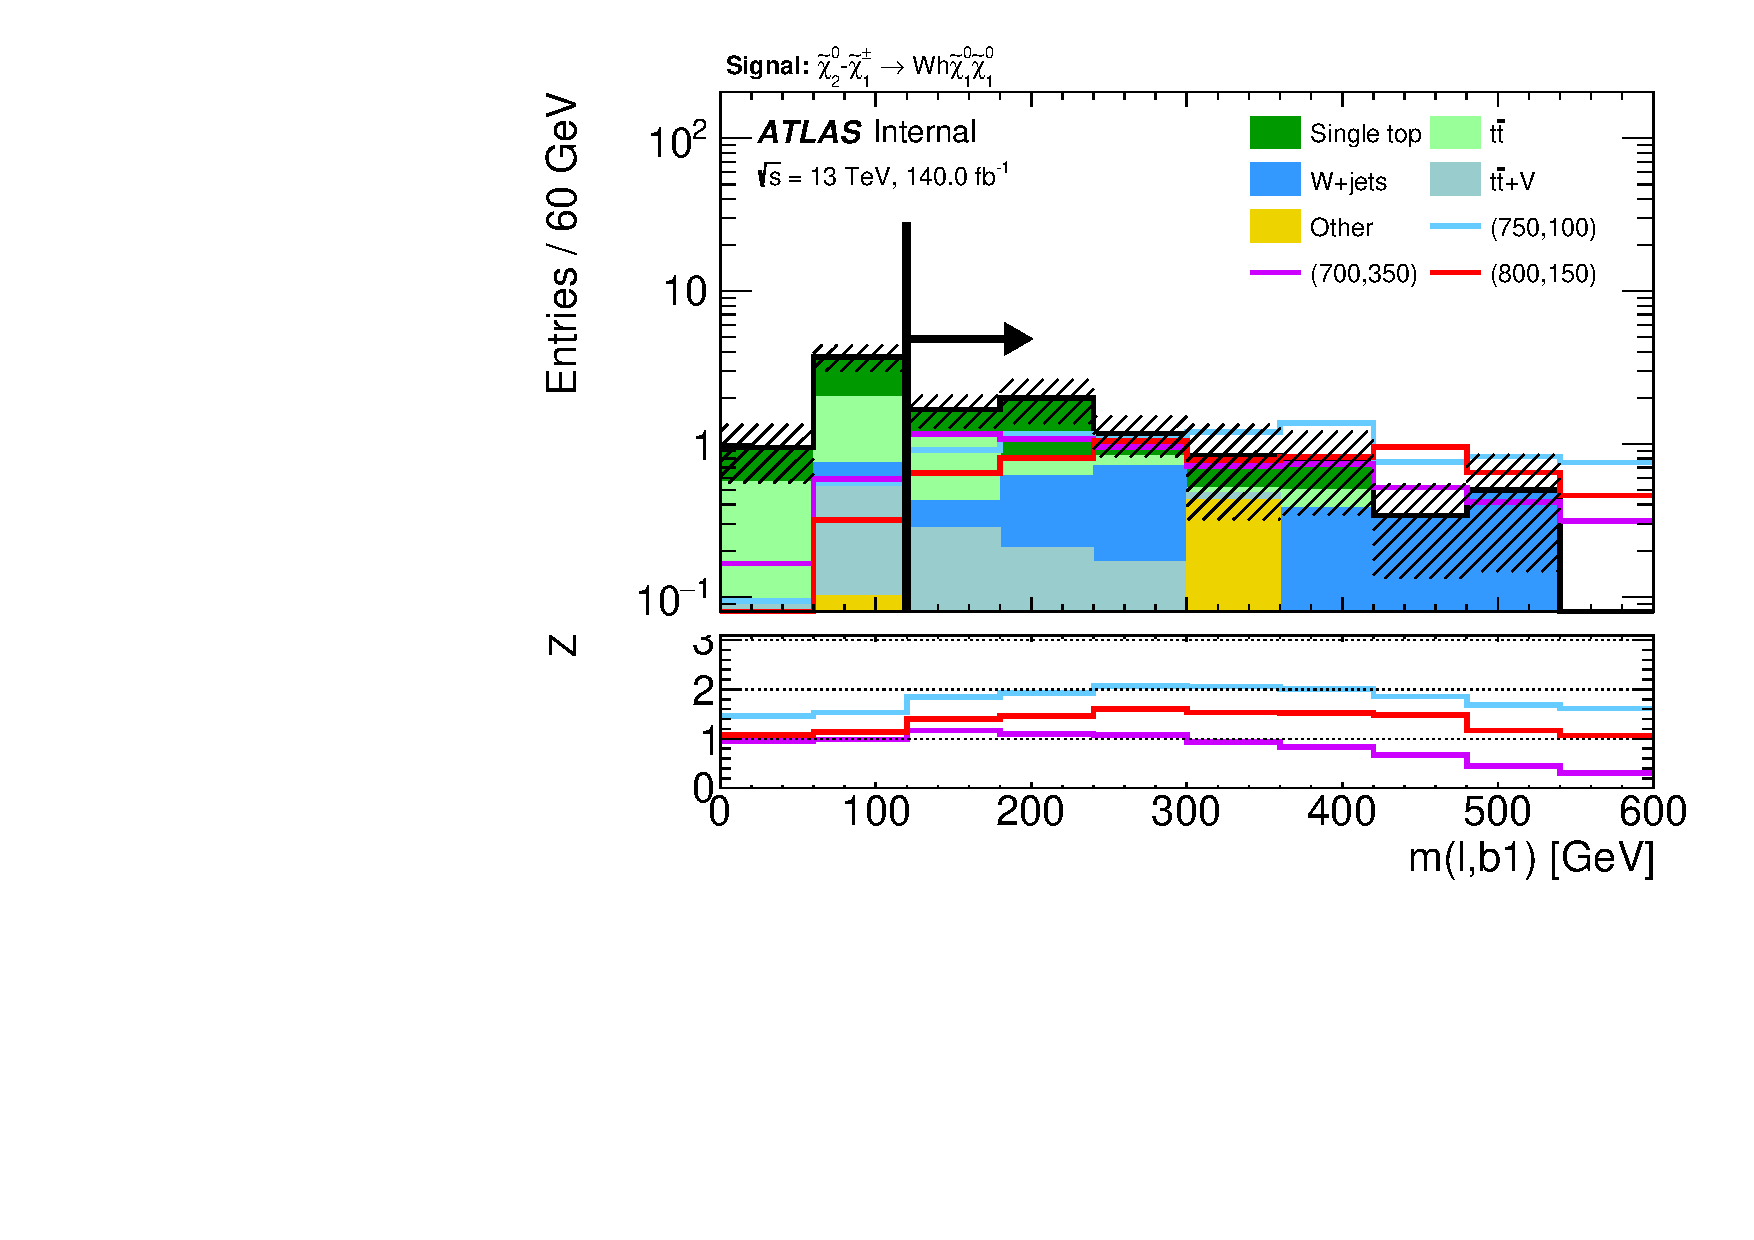
\includegraphics[width=\textwidth]{n1_SRHM_mct_bins/mlb1.pdf}
		\caption{\label{fig:Wh_reopt_second_round_n1_srhm_mlb1}}
	\end{subfigure}%
	\begin{subfigure}[b]{0.4\linewidth}
		\centering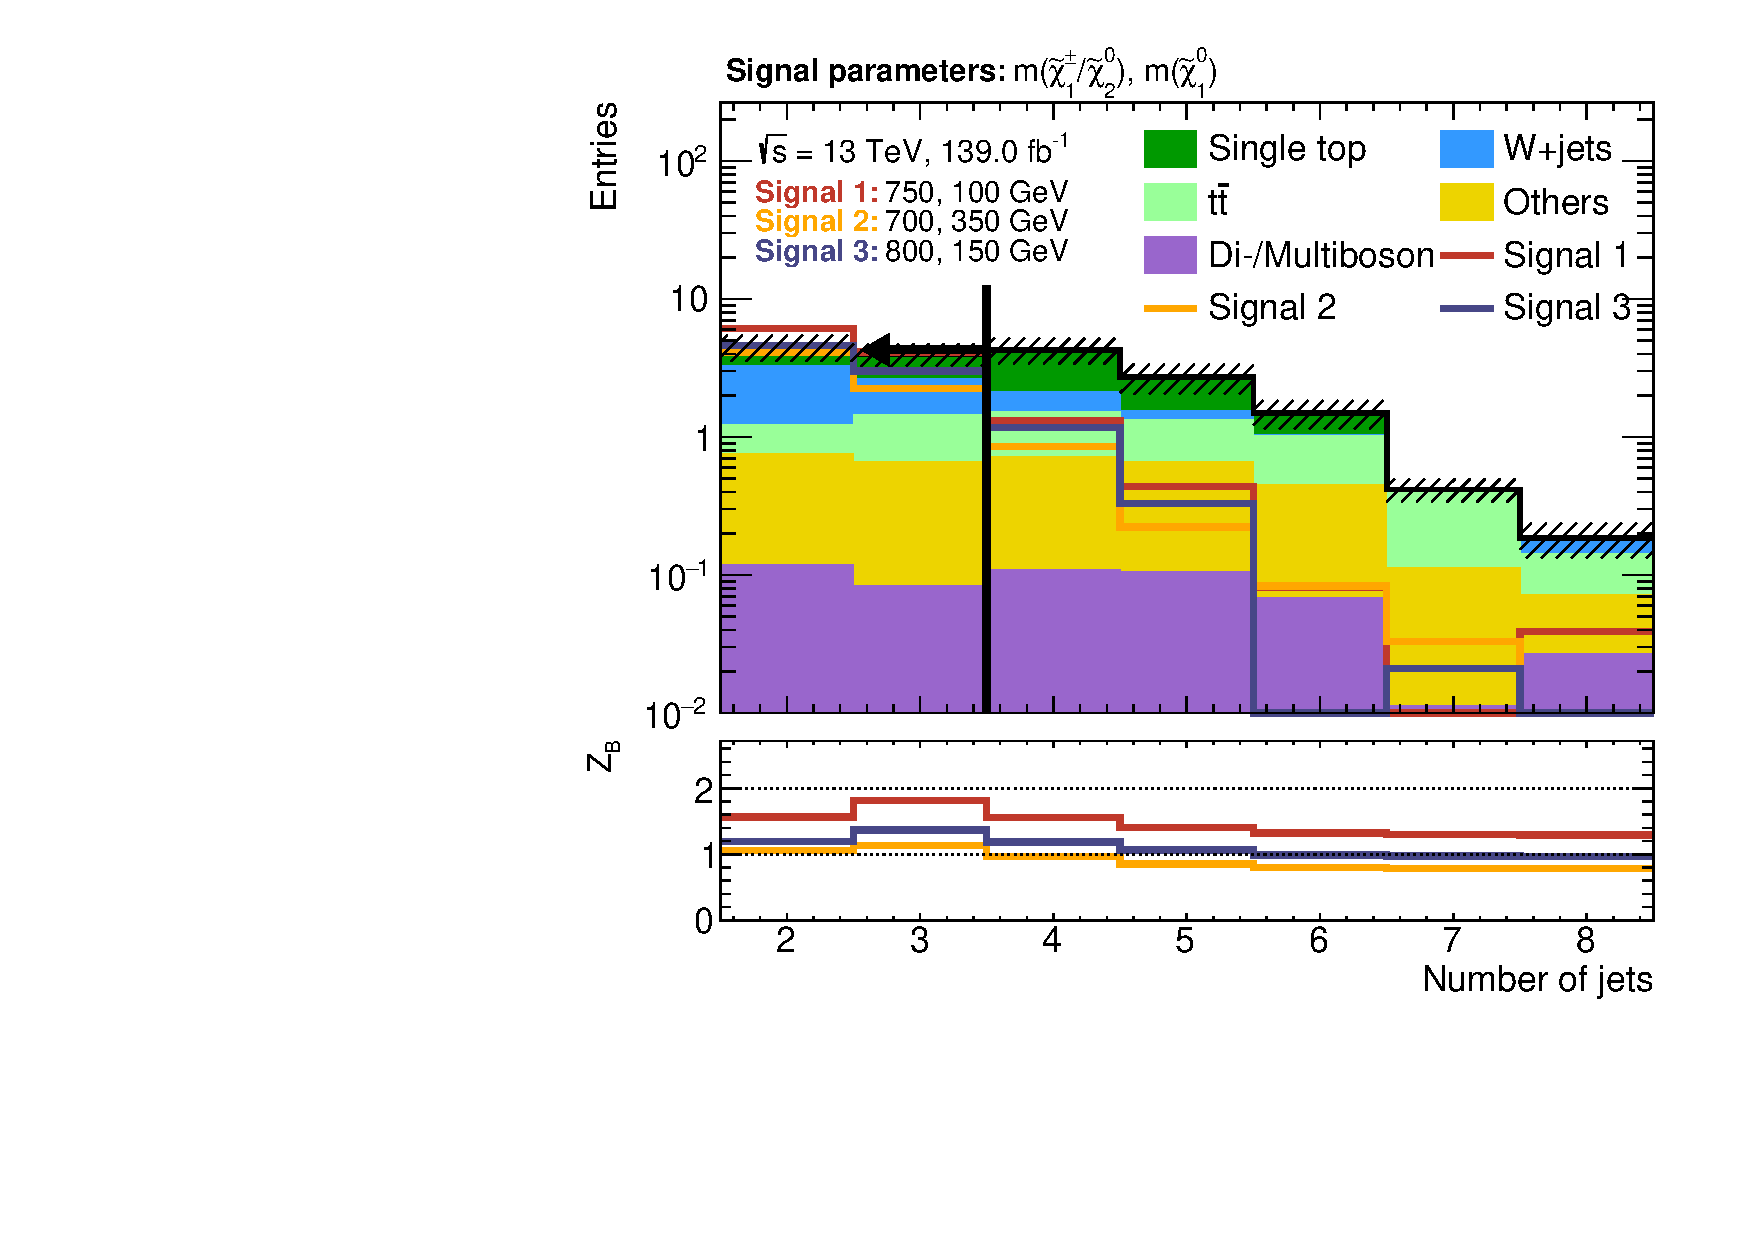
\includegraphics[width=\textwidth]{n1_SRHM_mct_bins/nJet30.pdf}
		\caption{\label{fig:Wh_reopt_second_round_n1_srhm_njet}}
	\end{subfigure}
	\caption{N-1 plots for the SR HM, with exemplary signal points and all $\mct$ bins included. In all figures except \figname~\subref{fig:Wh_reopt_second_round_n1_srhm_mct}, the significance in the lower pad is obtained by summing up all the events in the direction of the cut arrow and includes 30\% uncertainty as well as MC statistical uncertainty. In \figname~\subref{fig:Wh_reopt_second_round_n1_srhm_mct} the significance is only computed on a bin-by-bin basis, \ie not summing up all events in the direction of the cut arrow.}
	\label{fig:Wh_reopt_second_round_n1_srhm}
\end{figure}




